% !TeX spellcheck = en_US


\begin{frame}
	Recommended reading:\\
	\begin{itemize}
		\item Lectures in \cite{TreBau}: 6,7,8 for $QR$; 20,21 for $LU$; 23 for $LL^\top$
		\item Section I.4 in \cite{StrangData}
		\item Sections 2.6, 2.7 in \cite{StrangLA_intro}
	\end{itemize}
	~\\~\\
	\textbf{References}
	\bibliographystyle{plain}
	\bibliography{../information/literature}
\end{frame}

\begin{frame}
	
	\Section{Solving Linear Systems with Direct Methods}
	
	\textbf{Aim:}
		\begin{center}
		\textit{	Given $A\in\mathbb{R}^{m\times n}$ ($m\neq n$ possible) and $b\in\mathbb{R}^m$,
			find $x\in\mathbb{R}^n$ such that\\
			$Ax=b.$}
	\end{center}
\Subsection{The Idea of ``Factor and Solve''}
A general theme in numerical mathematics is to reduce the general (possibly complicated) problem to one or more simpler problems with the help of transformations for which the property of interest is an invariant.\\~\\\small
\Hide{	\textbf{Simple cases:}\\ 
	\begin{itemize}
			\item $A = D =  \text{diag}(d_1,\ldots, d_n)$ diagonal
			\item $A = L$ (or $A = U$) lower (or upper) triangular system\\
			$\rightarrow$ backward/forward substitution (exercise!)\\
			\item $A = Q$ orthogonal \\
			$\rightarrow$ $A^{-1} = Q^\top$ \\
			\item $A$ has special structure: tridiagonal/banded, Toeplitz, circulant,...
		\end{itemize}
~\\
\textbf{General case:}\\
\begin{itemize}
	\item[] Assume $A = F_1   \cdots F_k$, where each factor $F_i \in \{D, L, U, Q\}$, then formally
	$$ x = F_k^{-1}\cdots F_1^{-1} b,$$
	where each solving step $F_i^{-1}$ can easily be performed.\\~\\
\end{itemize}

{\small (\textit{Remark:} ``direct'' $=$ finitely many steps to obtain the solution (typically operating on dense arrays))}\\~\\}
\end{frame}

\begin{frame}
	~\\		
	\textbf{Separate: Factorization and Solution!}\\
	~\\	
	\begin{itemize}
		\item Since the \textit{factorization} (\textit{elimination/triangularization/orthogonalization}) step is typically much more expensive than the \textit{solution} step, it makes sense to perform them separately, if the same matrix $A$ is used for multiple right-hand sides $b$.\vspace{0.5cm}
		\item The number of factors in a decomposition is the number of systems to be solved in the \textit{solution} step.\vspace{0.2cm}
		From the factors we may also gain information about the
		\begin{itemize} \normalsize
			\vspace{0.15cm}\item the image and kernel of $A$
			\vspace{0.15cm}\item \text{invertibility} of the matrix $A$ in case $m=n$ 
			\vspace{0.15cm}\item \text{solvability} of the system (i.e., the cardinality $|S|$ of the solution set $S$)
		\end{itemize} \vspace{0.5cm}
		\item We will have a look at the following decompositions
		\begin{itemize} \normalsize
			\item $A = QR$ (two systems to be solved)
			\vspace{0.15cm}\item $A = P^TLU$ (three systems to be solved)
			\vspace{0.15cm}\item $A = LL^T$ (two systems to be solved)
		\end{itemize} 
	\end{itemize}
\end{frame}

\begin{frame}
	~\\~\\
		\textbf{Never compute the inverse!}~\\~\\
	\begin{itemize}
		\item There are only very rare occasions, where an inverse matrix $A^{-1}$ is needed. In most cases, one needs inverse matrix times a vector, i.e., $A^{-1}b$.	\vspace{0.2cm} 
		\item For computing the inverse of an $(n \times n)$-matrix $A$ we have to solve $n$ linear systems:\\
		\Hide{
		\begin{equation}\label{eq:compute-inverse}
		  A \cdot [x_1,\ldots, x_n]  = \idMat,
		\end{equation}
		where the $x_j \in \Rn$ are the unknown columns of the inverse of $A$. In practice, this is typically done by computing a factorization of $A$, which is then used to solve these $n$ linear systems in \eqref{eq:compute-inverse} (see, e.g., the LAPACK routine \texttt{getri}).}
		\vspace{0.5cm}		
		\item Thus, never do
		$$\texttt{ x = inv(A) @ b}$$ instead of
		$$\texttt{ x = solve(A, b)}.$$
	\end{itemize}
\end{frame}


\begin{frame}[c]
\hspace*{1.5cm}	\Subsection{The Gram-Schmidt Algorithm and the $QR$ decomposition}
\end{frame}	

\begin{frame}
\Subsubsection{Projectors}	 
For a fixed vector $x \in \Rn\setminus\{0\}$ we have derived the orthogonal projection onto its span by
\begin{equation*}
 \text{proj}_x(y) 
 = \frac{x}{\|x\|_2} \cdot \frac{x^\top y}{\|x\|_2}
 =  \frac{xx^\top}{x^\top x} \cdot y
 =: P_x y,
\end{equation*}
where $P_x := \frac{xx^\top}{x^\top x}\in \Rnn$.\\
~\\
\Hide{We now collect some properties of this matrix:
\begin{itemize}
	\item $\im(P_x) = \spann(x)$ (note that all columns are multiples of $x$) and thus $\rank(P_x) = 1$
	\item $P_x$ orthogonally projects a vector $y \in \Rn$ onto the linear subspace $\im(P_x)= \spann(x)$
	\item Idempotent: 
	$$P_x^2 := P_x\cdot P_x = \frac{xx^\top}{x^\top x} \cdot \frac{xx^\top}{x^\top x} = \frac{x(x^\top x) x^\top}{(x^\top x)^2}  = \frac{xx^\top}{x^\top x} = P_x .$$
	  $\rightarrow$ In words: Projecting multiple times is the same as projecting once. \\~\\
	  We make this a definition:
	  \begin{definition}[Projector] \label{def:projector}
	   A matrix $P \in \Rnn$ is called \textbf{projector} if $P^2=P$.
	  \end{definition}
\end{itemize}}
\end{frame}



\begin{frame}
	\Hide{
	\begin{example}[Projectors]~\\
		\begin{itemize}
			\item $x = (1,0)^\top, P_x = ...$
			\item $x= (1,1)^\top, P_x = ...$
			\item For $\alpha\in\R$ consider $P_\alpha =\begin{pmatrix}
				1 & \alpha\\
				0 & 0
			\end{pmatrix}$  (exercise sheet)
		\end{itemize}
	\end{example}
}
\end{frame}


\begin{frame}
	For any projector $P \in \Rnn$ we can show: 
	\begin{lemma}[Projector Properties]\label{lem:projector}
		Let  $P \in \Rnn$ be such $P^2 = P$, then
		\begin{itemize}
			\item[i)] \color{satzrot}$\im P = \ker (I-P)$,
			\item[ii)] \color{satzrot}$\ker(P) \cap \ker(I-P) = \{0\} $,
			\item[iii)] $(I-P)$ is also a projector,
			\item[iv)] $\forall y \in \Rn~ \exists_1 v \in \im(P), r \in \im(I-P)\colon ~y = v +r $,\\
			with other words, the mapping $\im(P) \times \im(I-P) \to   \Rn, (v,r) \mapsto v +r$ is bijective.
		\end{itemize}
	\end{lemma}
\Hide{	\begin{proof}~\\ 
		\begin{itemize}
			\item[i)] $\subseteq$: For $y=Px$ we find $(I-P)y = Px - P^2x = 0$.\\
			$\supseteq$: For $y \in  \ker(I-P)$ we have $y = (I-P + P)y = 0 + Py \in \im(P)$. 
			\item[ii)] Let $Px = 0 $ and $(I-P)x = 0$, then $x = (I-P + P)x = 0 + 0 = 0$.
			\item[iii)] $(I-P)^2 = I - 2P + P^2 = I -2P+P = I-P$.
			\item[iv)] Let $y \in \Rn$.\\
			Existence: Choose $v=Py \in  \im(P)$ and $r=(I-P)y \in \im(I-P)$, then we find 
			$$  v +r = Py + (I-P)y = y .$$
			Uniqueness: We assume there is another pair $\tilde{v} \in \im P= \ker(I-P)$ and $\tilde{r}\in \im(I-P)=\ker(P)$ with $y = \tilde{v} + \tilde{r}$. Since the kernel of matrix is a linear subspace (therefore closed under linear combinations), also $(v- \tilde{v})\in\ker(I-P)$ and $(r- \tilde{r})\in\ker(P)$. Now observe
			$0 = y-y = v- \tilde{v} + r -\tilde{r}. $
			Multiplying with $P$ yields
			$$0 = P(v- \tilde{v}) + P(r -\tilde{r})= P(v- \tilde{v}) ~~~\Rightarrow ~~~(v- \tilde{v}) \in \ker(P) \cap \ker(I-P) = \{0\} . $$
			Multiplying with $I-P$ yields
			$$0 = (I-P)(v- \tilde{v}) + (I-P)(r -\tilde{r})= (I-P)(v- \tilde{v}) ~~~\Rightarrow ~~~(r -\tilde{r}) \in \ker(I-P) \cap \ker(P) = \{0\}  .$$
			Thus $v = \tilde{v}$ and $r = \tilde{r}$. 
		\end{itemize}
	\end{proof}} 
\end{frame}


\begin{frame}
Remark:\\~\\ In view of Lemma \ref{lem:projector} iv) we say that $\Rn$ is the direct sum of the subspaces $\im(P)$ and $\im(I-P)$. Each vector $y \in \Rn$ uniquely splits into the additive components $v$ and $r$. Due to i) and iii) of this lemma, also the same is true for the subspaces  $\im(P)$ and $\ker(P)$.\\
~\\
\Hide{We now continue with properties of $P_x$:
Symmetry: $$P_x^\top = \frac{(xx^\top)^\top }{x^\top x}  = \frac{(x^\top)^\top x^\top }{x^\top x} = \frac{xx^\top}{x^\top x} = P_x .$$\\~\\
	 In general we define:
	\begin{definition}[Orthogonal Projector] \label{def:ortho-projector}
	A matrix $P \in \Rnn$ is called \textbf{orthogonal projector} if $P^2=P$ and $P^\top = P$. 
	\end{definition}	
For any orthogonal projector (such as $P_x$) one can show:
\begin{lemma}[Orthogonal Projector Properties]\label{lem:ortho-projector}
	Let  $P \in \Rnn$ be such $P^2 = P$ and $P^\top = P$, then
	$$\im P \bot  \im (I-P).$$
\end{lemma}
\begin{proof}
	From Lemma \ref{lem:projector} and Lemma \ref{lem:ortho-fundamental-subspaces} (1.45) as well as the symmetry of $P$ (and thus $I-P$) we find
	$$ \im(P) = \ker(I-P) = \ker((I-P)^\top) = \im(I-P)^\bot .$$
\end{proof}
In view of Lemma \ref{lem:projector} iv) we find for an orthogonal projector, that the  components $v \in \im( P)$ and $r \in \ker(P)$ are orthogonal to each other.} 
\end{frame}


\begin{frame}
\textbf{Orthogonal Projection with Orthonormal Basis}\\~\\
Let us now consider more than just one vector. In fact, let $q_1,\ldots, q_r \in \Rm$ be orthonormal; thus $r \leq m$. Then let us define the matrices
\begin{align*}
 \widehat{Q} &:= [q_1,\ldots, q_r] \in \R^{m \times r},\\
 P:=&P_{q_1,\ldots, q_r } := \widehat{Q}\widehat{Q}^\top  \in \Rmm.
\end{align*}
Attention: For $r < m$, $\widehat{Q}$ is not an orthogonal matrix and thus $ P = \widehat{Q}\widehat{Q}^\top \neq I$ in general. However, for the Gramian matrix which collects all possible pairs of inner products we have $ \widehat{Q}^\top\widehat{Q} = I$ ($\widehat{Q}^\top$ is only a left-inverse).\\~\\
\Hide{We find the following properties of $P=P_{q_1,\ldots, q_r }$:
\begin{itemize}
	\item Sum of rank--one (orthogonal) projectors:\\
	 $$ P= \sum_{j=1}^r q_j q_j^\top = \sum_{j=1}^r P_{q_j} .$$
	 \item Orthogonal projector:
	 \begin{align*}
	  & P^2 = \widehat{Q}(\widehat{Q}^\top\widehat{Q})\widehat{Q}^\top = \widehat{Q}\widehat{Q}^\top = P\\
	  & P^\top = (\widehat{Q}\widehat{Q}^\top)^\top = (\widehat{Q}^\top)^\top\widehat{Q}^\top = P
	 \end{align*}
	 \item $P$ projects on the image of $\widehat{Q}$:
	 In fact, by Lemma \ref{lem:kerImProducts} (1.47) ii) (with $\im(\widehat{Q}^\top)=\R^r$) we find
	  $$\im(P) = \im(\widehat{Q}\widehat{Q}^\top) = \im(\widehat{Q}).$$
	  In particular: $\rank(P) = r$.
\end{itemize}}
\end{frame}

\begin{frame}
\Hide{	\begin{itemize}
		\item By Lemma \ref{lem:projector} i)+iii) and Lemma \ref{lem:kerImProducts}(1.47) i) (with $\ker(\widehat{Q}) = \{0\}$) we find 
	     \begin{align*}
	          \im (I-P) = \ker(P) = \ker(\widehat{Q}\widehat{Q}^\top) = \ker (\widehat{Q}^\top) 
	     \end{align*}
	    \item In Lemma \ref{lem:ortho-projector} we recover Lemma \ref{lem:ortho-fundamental-subspaces} (1.45):
	    \begin{align*}
	     \im(P)\bot  \im (I-P)
	      ~~~\Leftrightarrow ~~~ 
	      \im(\widehat{Q}) \bot \ker (\widehat{Q}^\top) 
	    \end{align*}
		\item By Lemma \ref{lem:projector} iv) we have 
		\begin{align*}
		 \forall y \in \Rn~ \exists_1 v \in \im(P)=&\im(\widehat{Q}), r \in \im (I-P) =\ker(\widehat{Q}^\top)\colon\\ 
		 y &= v + r \\
		 & = Py + (I-P) y\\
		 & = \widehat{Q}\widehat{Q}^\top y + (I- \widehat{Q}\widehat{Q}^\top) y
		\end{align*}
		where $v$ is the orthogonal projection of $y$ onto $\im(\widehat{Q})$ and $r$ the orthogonal residual vector; the components are orthogonal, i.e., 
		$$(v,r) = v^\top r = 0.$$
	\end{itemize}}
\end{frame}

\begin{frame}
	\begin{example}Let us consider:\\
		$$q_1 = \frac{1}{\sqrt{2}}(1,1,0)^\top, q_2 =  \frac{1}{\sqrt{2}}(-1,1,0), y=(0,1,1)^\top  \in \R^3 $$
\Hide{		Then
		$$P = \widehat{Q} \widehat{Q}^\top = \begin{pmatrix}
		 1 & 0 & 0 \\ 0 & 1 & 0 \\ 0 & 0 & 0
		\end{pmatrix} $$
		So that for $y = (y_1, y_2, y_3)^\top \in \R$ we obtain
		$$ Py = \begin{pmatrix}
		y_1\\y_2\\0
		\end{pmatrix}= \begin{pmatrix}
		0\\1\\0
		\end{pmatrix},$$
		i.e., as expected the orthogonal projection onto the $x_1/x_2$-plane (=$\im(\widehat{Q})$).}
	\end{example}
\end{frame}
 
\begin{frame}
	 \textbf{Orthogonal Projection with Arbitrary Basis}\\~\\
	 Let $a_1,\ldots, a_n$ be linearly independent vectors in $\Rm$ ($m \geq n$) and let us put the vectors into a matrix $A = [a_1,\ldots, a_n] \in \Rmn$.\\
	 
	 \textit{How to define an orthogonal projector on the image of $A$?}\\~\\
\Hide{	 Let us first recall that $\im(A) \bot \ker(A^\top)$ by Lemma \ref{lem:ortho-fundamental-subspaces} (1.45).
	 Thus we are looking for a matrix $P \in \Rmm$ such that
	 \begin{align*}
	  &\forall b \in \Rm\colon ~Pb \in \im(A)~\text{, i.e.,} Pb = Ax~\text{for some $x$ to be determined}\\
	  &b - Pb \in \im(A)^\bot = \ker(A^\top)
	 \end{align*}
	 Combining these two gives
	 $$0 = A^\top(b - Pb)= A^\top(b - Ax)  =  A^\top b - A^\top Ax. $$
	 Then by Lemma \ref{lem:kernel-image} (1.46) i) we have $\ker(A^\top A) = \ker(A) = 0$, so that the Gram matrix $A^\top A$ is invertible, which yields
  	 $$ x = (A^\top A)^{-1}A^\top b $$
  	 and the orthogonal projection $b$ onto the image of $A$ is given by
  	 $$Ax =   A(A^\top A)^{-1}A^\top b =: Pb.$$
 	 Indeed we find, $P^2 = P$ and $P^\top = P.$ Also note that for $A=\widehat{Q}$ this collapses to $P = \widehat{Q}\widehat{Q}^\top$. Further note that this coincides with $P_x = x (x^\top x)^{-1} x^\top$.
 ~\\
 {\footnotesize -----\\ \textit{Remark: The final step to bridge between orthogonal projections and least squares, is to show the intuitive result that orthogonal projections are precisely those projections that produce the smallest residual $(I-P)b$. This is shown later in this course.}}}
\end{frame}

\begin{frame}
	\begin{example}Let us consider:\\
		$$a_1 = (1,1,0)^\top, a_2 =  (0,1,0), y=(0,1,1)^\top  \in \R^3 .$$
		We observe that $\im(A) = \im(\widehat{Q})$, so that we would expect the same projector as in the example above.\\
\Hide{		First we compute
		$$A^\top A = \begin{pmatrix}
		 2 & 1 \\ 1 & 1
		\end{pmatrix}. $$
		From $$A^\top A x = \begin{pmatrix}
		1 \\ 0
		\end{pmatrix} \Leftrightarrow x =  \begin{pmatrix}
		1 \\ -1
		\end{pmatrix} $$
		and 
		$$A^\top A x = \begin{pmatrix}
		0 \\ 1
		\end{pmatrix} \Leftrightarrow x =  \begin{pmatrix}
		-1 \\ 2
		\end{pmatrix} $$
		we find 
		$$(A^\top A)^{-1} = \begin{pmatrix}
		1 & -1 \\ -1 & 2
		\end{pmatrix}. $$
		And thus
		$$P = A (A^\top A)^{-1} A^\top =  \begin{pmatrix}
		1 & 0 & 0 \\ 0 & 1 & 0 \\ 0 & 0 & 0
		\end{pmatrix} .$$}
	\end{example}
\end{frame}

\begin{frame}
	\Subsubsection{A=QR from the (classical) Gram--Schmidt Algorithm}	
\Hide{\begin{center}
	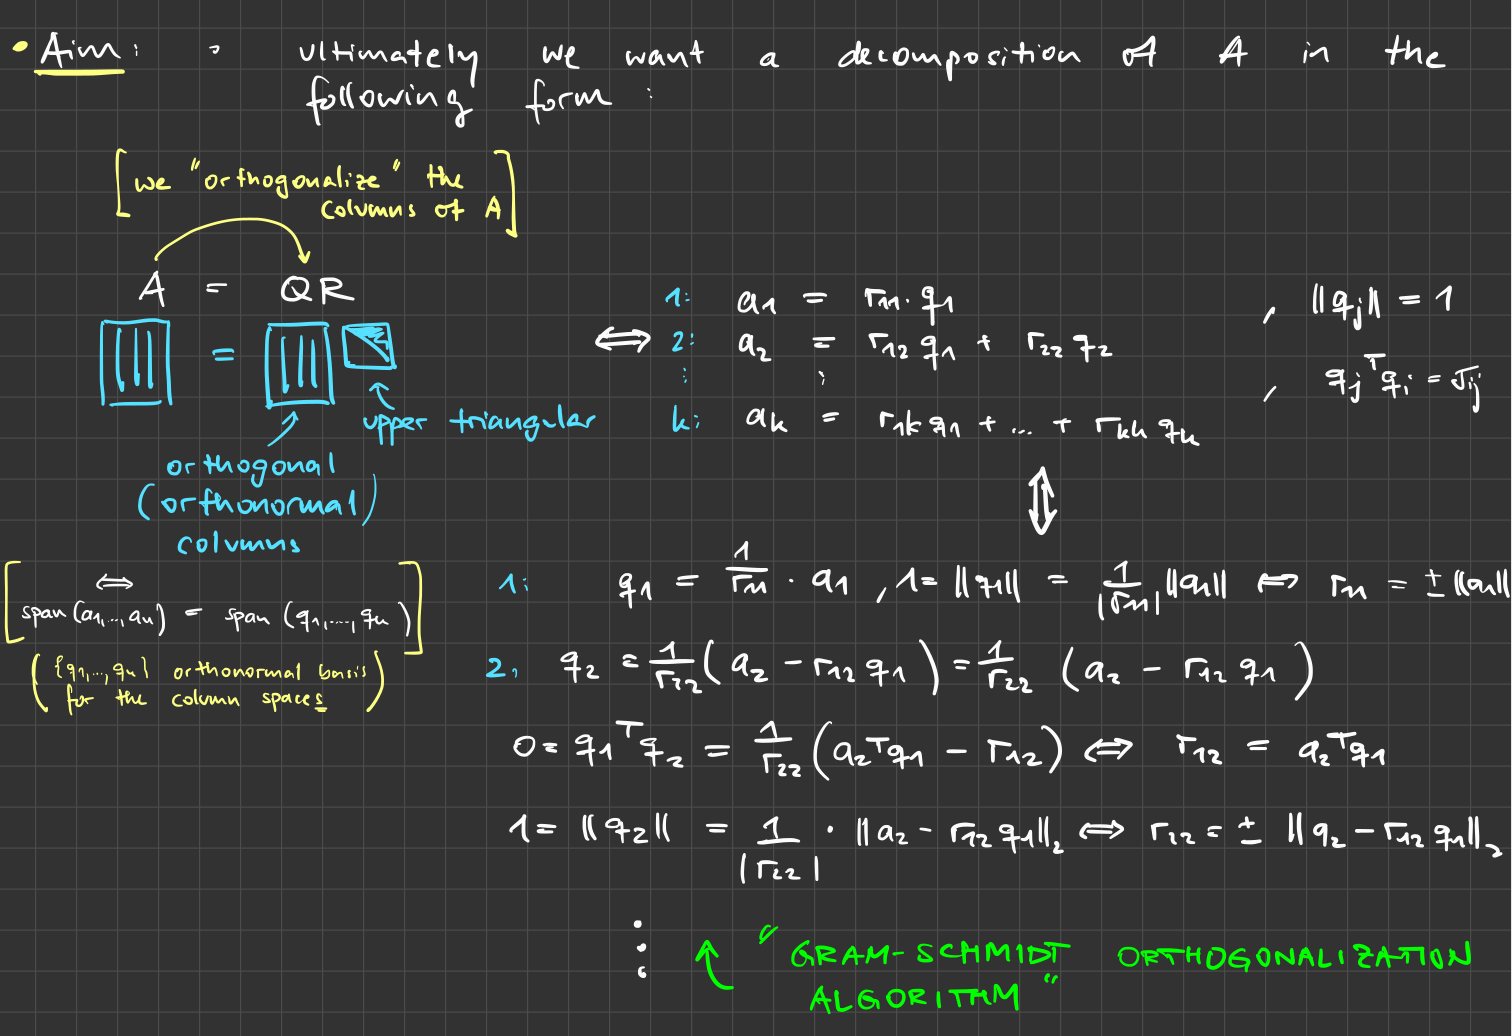
\includegraphics[width=0.94\linewidth]{content/Gram-Schmidt-Idea}
\end{center}}
\end{frame}


\begin{frame}[c]
\textbf{Classical Gram--Schmidt Orthogonalization Algorithm}\\~\\
\hspace*{1cm}
\begin{minipage}{0.8\textwidth}
\begin{algorithm}[H]
$r_{11} = \| a_1 \|$\\
$q_1 = \frac{a_1}{r_{11}}$\\
~\\
\For{ $k = 2, \dots, n$ }{ 
\For{ $\ell = 1,\dots, k-1$}{  
	$r_{\ell k} = a_k^\top q_\ell$	\\
 } 
		$\widetilde{q}_k = a_k - \sum _{\ell=1}^{k-1} r_{\ell k} \, q_\ell~~ {\color{cyan}= (I-P_{q_1,\ldots,q_{k-1}})a_k \in \im(\widehat{Q}_{k-1})^\bot}$\\
	$r_{kk} = \| \widetilde{q}_k \|$\\
	\If{$r_{kk} = 0$}{
		pick arbitrary $q_k \in \im(\widehat{Q}_{k-1})^\bot = \ker(\widehat{Q}_{k-1}^\top)$	\\
	    {\color{gray}// for example by solving $\widehat{Q}_{k-1}^\top q_k = 0$ and normalizing}
}\Else{$q_k = \frac{\widetilde{q}_k}{r_{kk}}$}
}
{\color{gray}// For full QR:}\\
Fill up columns of $\widehat{Q}:= \widehat{Q}_n$ with $(m-n)$ orthonormal vectors of $\ker(\widehat{Q}_{k-1}^\top)$\\
Fill up rows of $\widehat{R} := (r_{ij})$ with $(m-n)$ zero rows
\end{algorithm}
\end{minipage}
~\\
\textit{\color{cyan} Observation: This algorithm successively orthogonalizes the columns of $A$!}
 \end{frame}


\begin{frame}
	These ideas lead to\\
	\begin{theorem}[QR decomposition]\label{theo:qr¸}
		Let $A\in\R^{m\times n}$ with $m \geq n$, then there exists a matrix $\widehat Q\in\R^{m\times n}$ with orthonormal columns and an upper triangular matrix $\widehat R\in\R^{n\times n}$ such that
		$$A=\widehat Q \widehat R.$$
		{\color{defgruen} We call this the \textbf{\underline{reduced} QR decomposition} of $A$.}\\~\\
		One can extend the columns of $\widehat Q$ with orthonormal columns to obtain an orthogonal matrix $Q\in\R^{m\times m}$ and the rows of $\widehat R$ by zero rows to obtain a matrix $R =\begin{pmatrix}
		\widehat{R}\\0
		\end{pmatrix}\in \R^{m\times n}$ and thereby obtain
		$$A = QR .$$
		{\color{defgruen} We call this the \textbf{QR decomposition} of $A$.}
	\end{theorem}\vspace{-0.1cm}
	\Hide{
		\begin{proof}\small
		Sketch: First note that by construction $\spann(a_1,\ldots, a_k) = \spann(q_1,\ldots, q_k)$ for all $1\leq k \leq n$ and $q_1,\ldots, q_k$ orthonormal (exercise: verify this by an induction proof).\\		
		If $\ker(A) = \{0\}$ (independent columns), then for all $1\leq k \leq n$ we have $$a_k \notin \spann(a_{1},\ldots, a_{k-1}) = \spann(q_{1},\ldots, q_{k-1}) $$  and thus for the residual of the projection
		$$\widetilde{q}_k = (I-P_{q_1,\ldots,q_{k-1}})a_k\neq 0$$
		so that $r_{kk} \neq 0$. Thus the classical Gram-Schmidt algorithms produces $\widehat{Q}$ and $\widehat{R}$ so that $A = \widehat{Q}\widehat{R}$.\\
		If columns of $A$ are dependent, then there are $k$ for which 
		$$a_k \in \spann(a_{1},\ldots, a_{k-1}) = \spann(q_{1},\ldots, q_{k-1})$$ so that the residual is $\widetilde{q}_k = (I-P_{q_1,\ldots,q_{k-1}})a_k = 0$, thus we pick an arbitrary vector in $q_k \in \im(\widehat{Q}_{k-1})^\bot = \ker(\widehat{Q}_{k-1}^\top)$ and continue.
	\end{proof}}
\end{frame}
\begin{frame}
	\begin{example}~\\
\Hide{	 \begin{center}
	 	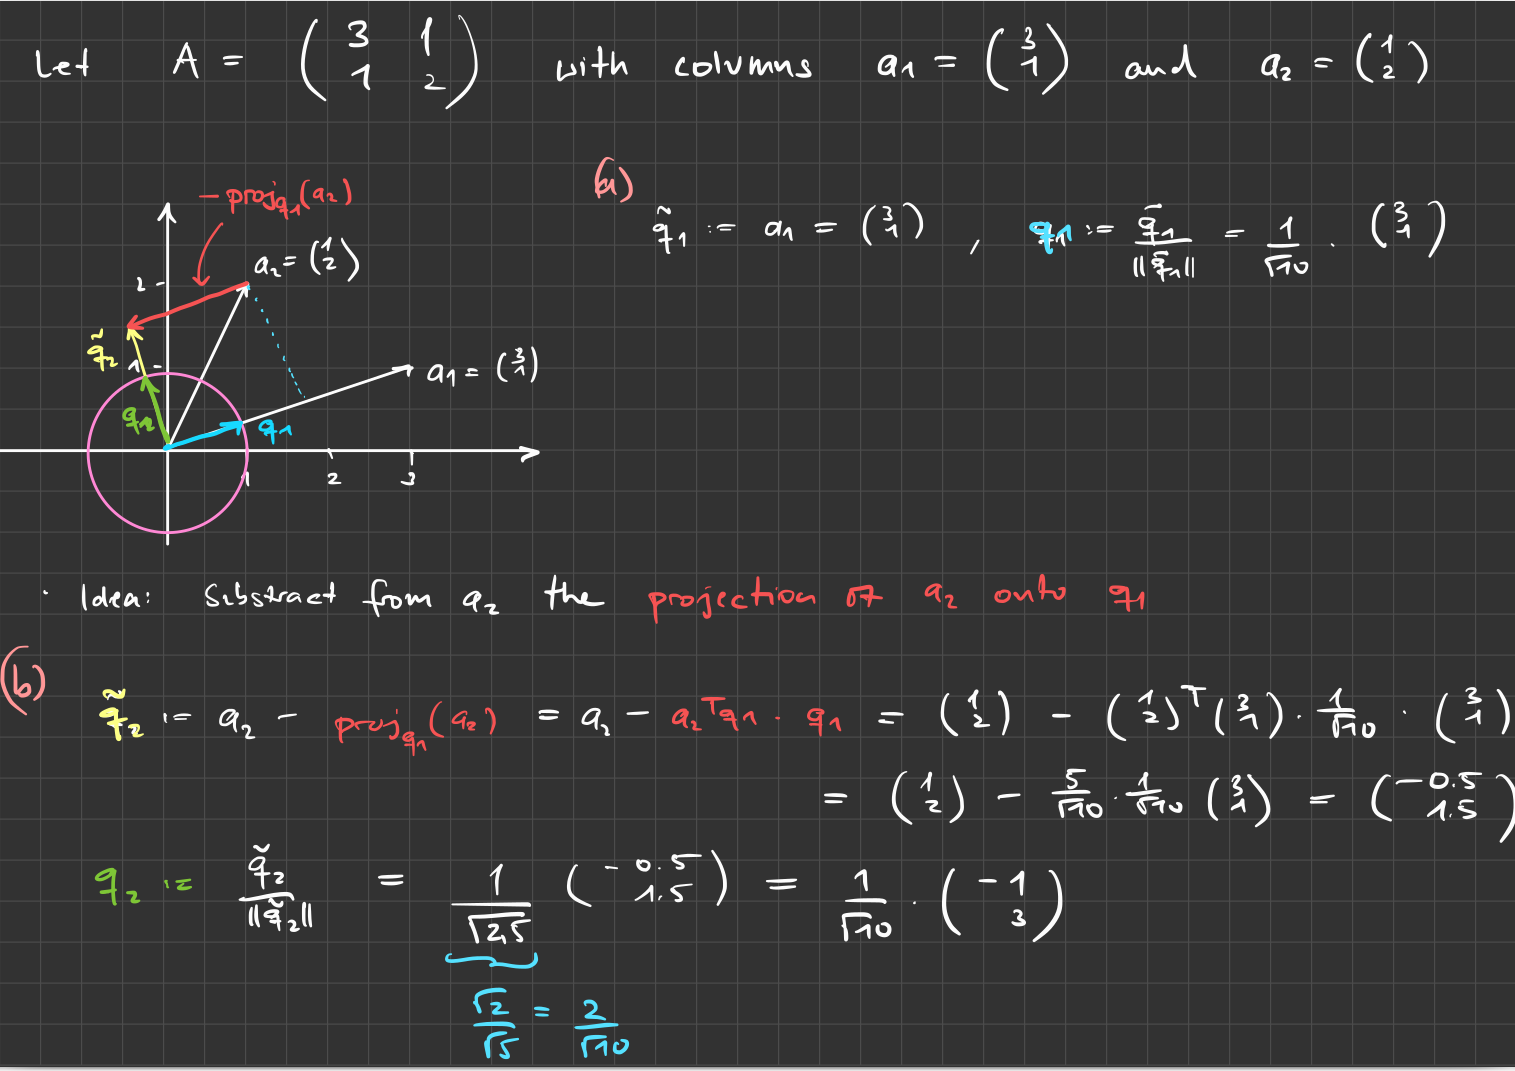
\includegraphics[width=0.95\linewidth]{content/Gram-Schmidt-Example-1}
	 \end{center}}
	\end{example}
\end{frame}
\begin{frame}
	\Hide{	 \begin{center}
		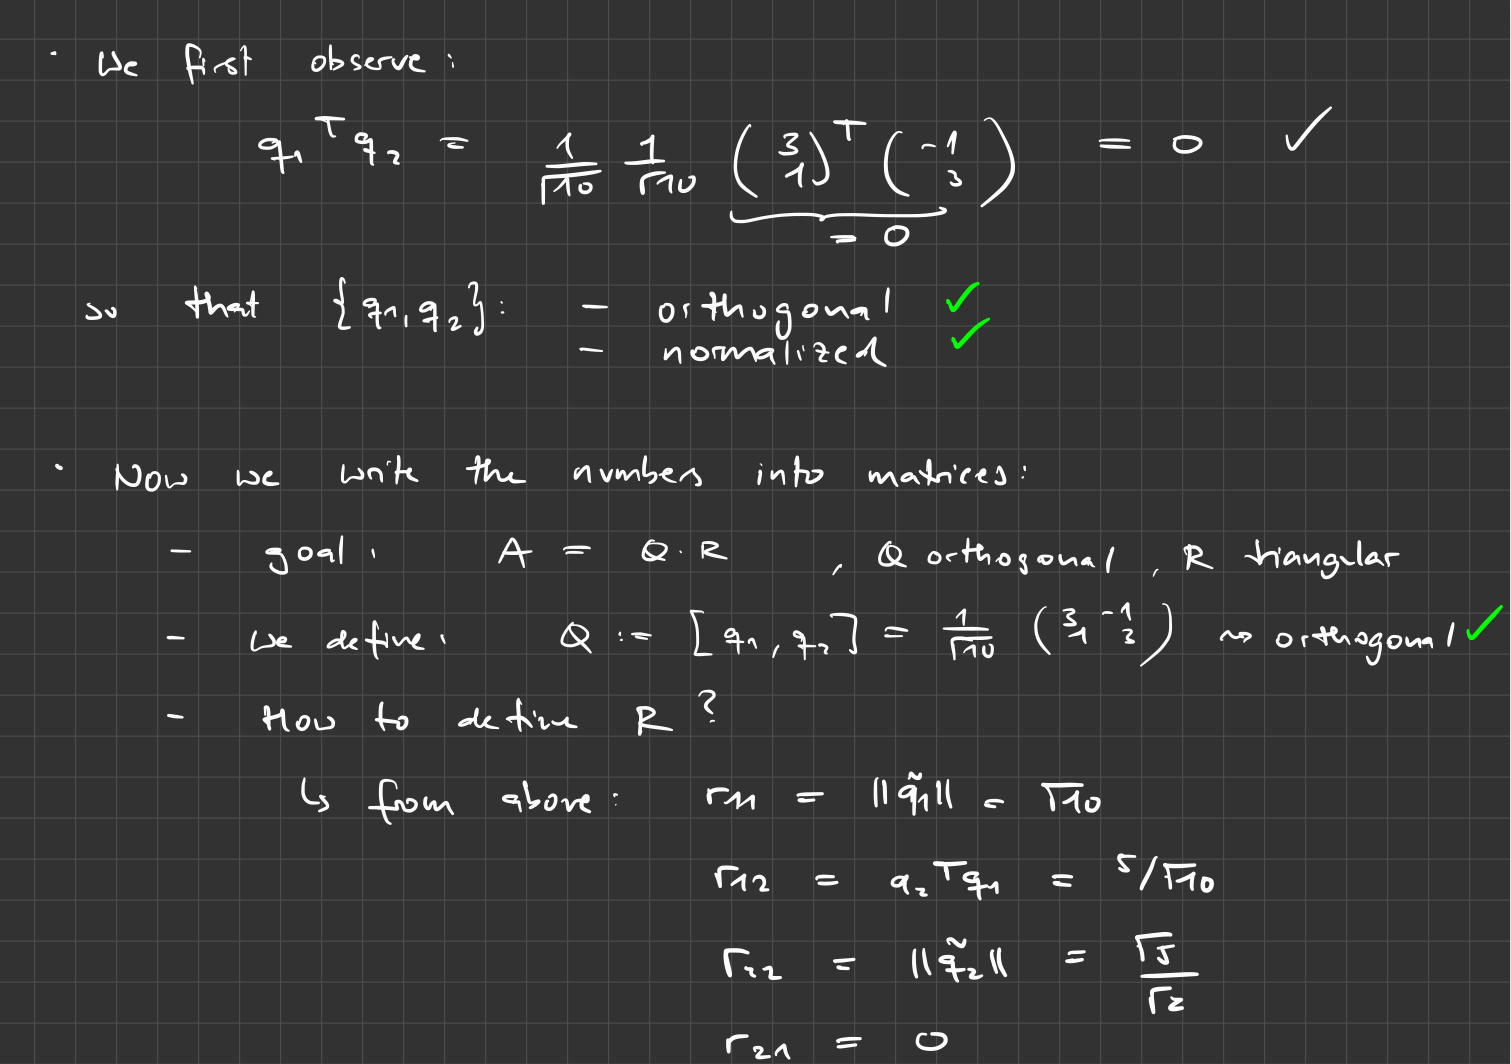
\includegraphics[width=0.95\linewidth]{content/Gram-Schmidt-Example-2}
	\end{center}}
\end{frame}
\begin{frame}
\Hide{	\begin{center}
		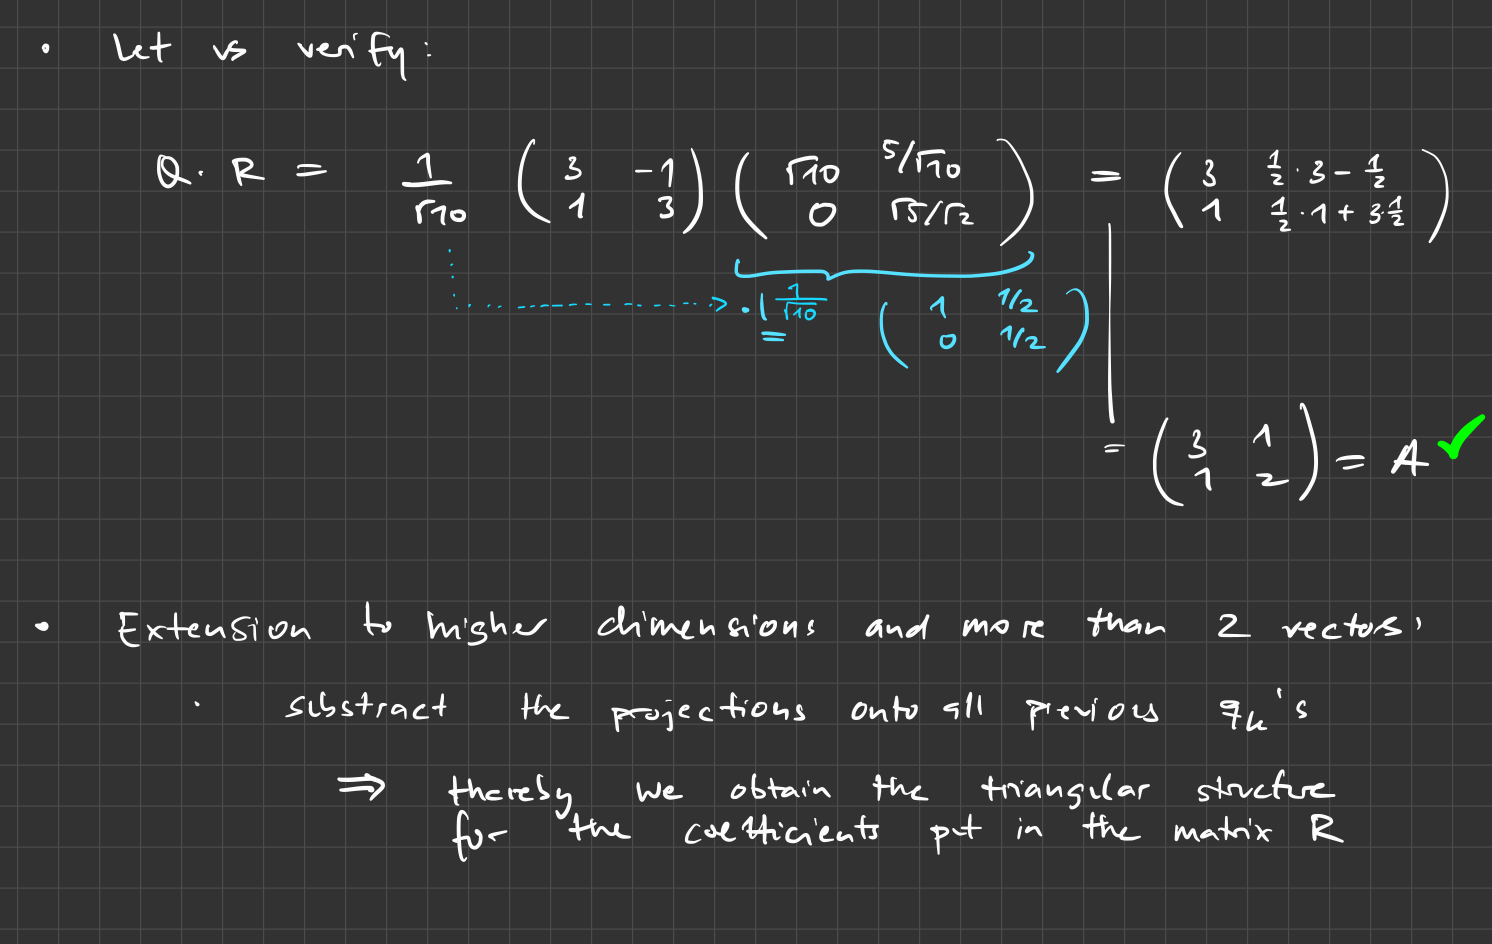
\includegraphics[width=0.95\linewidth]{content/Gram-Schmidt-Example-3}
	\end{center}}
\end{frame}





\begin{frame}
	Let $m \geq n$.\\
	~\\
	\textbf{(1) Factorization}~\\
Gram-Schmidt orthogonalization algorithm, Householder reflections or Givens Rotations can be used.\\~\\
	\textit{In Python}
	$$Q, R = \texttt{scipy.linalg.qr(A)} $$
	~\\
	\textit{or for the reduced version run }
	$$\widehat{Q}, \widehat{R}  = \texttt{scipy.linalg.qr(A, mode="economic")}$$
	~\\
	\textbf{(2) Solving}~\\
	\Hide{
	Let us consider the reduced $QR$ decomposition $\widehat{Q}\widehat{R}=A$. Then project $b$ on the image of $A$ by $\widehat{Q}\widehat{Q}^\top b$. Then we obtain the solvable auxiliary problem
		\begin{align*}
	Ax=\widehat{Q}\widehat{Q}^\top b~~\Leftrightarrow~~\widehat{Q}\widehat{R}x= \widehat{Q}\widehat{Q}^\top b~~
	\stackrel{{\color{cyan}\ker \widehat{Q} = \{0\} }}{\Leftrightarrow}~~\widehat{R}x = \widehat{Q}^\top b.
	\end{align*}
	Note that if $b \in \im(A)$ then $b= \widehat{Q}\widehat{Q}^\top b$, so that in this case we solve the original problem
	$$Ax=\widehat{Q}\widehat{Q}^\top b = b .$$
	~\\
%	 containing the first $n$ orthonormal columns of $Q$ and $\widehat{R} \in \Rnn$ with $R =\begin{pmatrix}
%	\widehat{R}\\0
%	\end{pmatrix} $. Since $\widehat{Q}^\top$ is a left--inverse of $\widehat{Q}$ (i.e., $\widehat{Q}^\top\widehat{Q} = I $), we find the  solution by
%	\begin{align*}
%	Ax=b~~\Leftrightarrow~~\widehat{Q} \widehat{R}x=b~~
%	\stackrel{{\color{cyan}\widehat{Q}^T\cdot |~,  \widehat{Q}\cdot | }}{\Leftrightarrow}~~\widehat{R}x = \widehat{Q}^\top b
%	\end{align*}
	\textit{In Python}
	$$\texttt{x = scipy.linalg.solve\_triangular(R, Q.T @ b)} $$
}
\end{frame}



\begin{frame}[c]
	\hspace*{1.5cm}	\Subsection{Gaussian Elimination and the $LU$ Decomposition}
\end{frame}	
\begin{frame}
	
	~\\~\\
		\textbf{(1) Factorization:} Row elementary operations \\~\\
		Apply transformations to $A$ (and $b$), which do not affect the solution $x$ (more precisely the solution set $S$ will not change), to bring $A$ into a simple form and collect all transformations on the fly.\\ 
	\begin{itemize}
		\vspace{0.3cm}\item the factorization \textbf{process} is known as \textit{Gaussian Elimination}
		\vspace{0.3cm}\item the \textbf{result} will be an invertible lower triangular matrix $L$, some sort of upper triangular matrix $U$ and an orthogonal (more precisely a permutation) matrix $P$, such that
		$$ A = P^T{\color{orange}LU}. $$ 	     
	\end{itemize}
		~\\
\textbf{(2) Solve:} Forward/Backward substitution \\
$$Ax = b \Leftrightarrow  Ux = L^{-1}Pb $$
\end{frame}

\begin{frame}
\textbf{~Example 1:} Frobenius Matrices\\~\\
$A=\begin{pmatrix}
1&3&5\\0&2&3\\2&4&6
\end{pmatrix},
~b=\begin{pmatrix}4\\2\\6\end{pmatrix}~~~~~~~~~~~~~
Ax=b~~\Leftrightarrow~~
\begin{matrix}
x_1&+3x_2&+5x_3&=4\\
~&2x_2&+3x_3&=2\\
2x_1&+4x_2&+6x_3&=6
\end{matrix}$
~\\
	\Hide{
			{\small
				~\\
				We apply the transformation: \textit{1) scaling one row and adding it to another row}\\
				\begin{align*}
				\left(\begin{array}{ccc|c}
				1&3&5&4\\
				0&2&3&2\\
				2&4&6&6
				\end{array}\right)
				\stackrel{\text{III'=III-2I}}{\Leftrightarrow}
				\left(\begin{array}{ccc|c}
				1&3&5&4\\
				0&2&3&2\\
				0&-2&-4&-2
				\end{array}\right)
				\stackrel{\text{III'=III+II}}{\Leftrightarrow}
				\left(\begin{array}{ccc|c}
				1&3&5&4\\
				0&2&3&2\\
				0&0&-1&0
				\end{array}\right)\\
				\textcolor{cyan}{
					A|b\hspace{1cm}\xrightarrow[L_1\cdot|]{}\hspace{1.7cm}L_1A~|~L_1b\hspace{1.5cm}\xrightarrow[L_2\cdot|]{}\hspace{1.3cm}L_2L_1A~|~L_2L_1b
				}
				\end{align*}
				$$
				\begin{matrix}
				\text{III)}~\Rightarrow~~x_3=0\\
				\text{II)}~\Rightarrow~~x_2=1\\
				\text{I)}~\Rightarrow~~x_1=1\\
				\end{matrix}~~\Rightarrow~~x=\begin{pmatrix}1\\1\\0\end{pmatrix}
				$$
%			
					\underline{Observation:}\\
					The transformations $L_i$ can be written as:
					$$
					L_1=
					\begin{pmatrix}
					1&0&0\\0&1&0\\{\color{orange}-2}&0&1
					\end{pmatrix},~
					L_2=
					\begin{pmatrix}
					1&0&0\\0&1&0\\0&{\color{orange}1}&1
					\end{pmatrix}
					$$
				Let us verify this for the first step
				\begin{align*}
				&L_1A~=~\begin{pmatrix}
				1&0&0\\0&1&0\\-2&0&1
				\end{pmatrix}
				\begin{pmatrix}
				1&3&5\\0&2&3\\2&4&6
				\end{pmatrix}
				=\begin{pmatrix}
				1&3&5\\0&2&3\\0&-2&-4
				\end{pmatrix},~~L_1b~=~\begin{pmatrix}4\\2\\-2\end{pmatrix}
				\end{align*}
			And since the transformations $L_i$ are injective (independent columns), after the first step, we obtain an equivalent linear system: \vspace*{-0.08cm}
			$$Ax=b~~\Leftrightarrow~~L_1Ax=L_1b$$
			}
	}
\end{frame}

\begin{frame}
	~\\
	\Hide{ 
		~\\
		\underline{All in all:}\\~\\
		By defining the upper triangular matrix $U:= L_2L_1 A$ and the lower triangular matrix $L:=L_1^{-1}L_2^{-1}$ we find 
		$$A = LU. $$
		~\\
		\underline{In general:}\\~\\
		If ``$A$ permits'', we obtain:
		\begin{align*}
		\underbrace{
			(L_{n-1}\cdots L_2L_1)}_{~\textit{(lower triangular + invertible)}}\cdot A = U
		~~~~~\Leftrightarrow~~~~~~
		~~A=LU,~~~~~L:=(L_{n-1}\cdots L_2L_1)^{-1}.
		\end{align*}
		
		~\\~\\
		Note:\\
		\begin{itemize}
			\item 		The lower triangular structure in the matrices $L_j$ is obtained by following a ``top to bottom'' approach.\\
			\item Thereby we also make sure that we ultimately obtain an ``upper triangular'' system.
		\end{itemize}
	}
\end{frame}

\begin{frame}
\textbf{Frobenius Matrices}\\~\\
\Hide{
	$$
	\underbrace{
		\begin{pmatrix}
		1&0&~&~&~&\cdots&0\\
		0&1&0&~&~&~&\vdots\\
		~&0&\ddots&0&~&~&~\\
		~&~&0&1&0&~&~\\
		~&~&0&\ell_{j+1,j}&\ddots&0&~\\
		\vdots&~&\vdots&\vdots&0&1&0\\
		0&\cdots&0&\ell_{m,j}&0&0&1
		\end{pmatrix}}_{=:L_j}
	\begin{pmatrix}
	--a_1--\\
	--a_2--\\
	\vdots\\
	--a_j--\\
	\vdots\\
	--a_m--
	\end{pmatrix}
	=\begin{pmatrix}
	--a_1--\\
	\vdots\\
	--a_j--\\
	\ell_{j+1,j}a_j+a_{j+1}\\
	\vdots\\
	\ell_{m,j}a_j+a_{m}
	\end{pmatrix}
	$$
\begin{itemize}
	\item 	If $L_j$ is defined in this way, then $\ell_{i,j}$ is the multiple for the $j$-th row which is then added to the $i$-th row.\\
	\item Since we want to produce zeroes underneath the diagonal element in our system, we choose $$\ell_{i,j}=-\frac{a_{ij}}{a_{jj}}~(a_{jj}\neq 0).$$
	~\\~\\
	\item[$\rightarrow$] We will now illuminate properties of such Frobenius matrices which come in handy when analyzing the Gaussian elimination procedure!
\end{itemize}
} 
\end{frame}
\begin{frame}
	\textbf{Properties}\\
	\begin{lemma}\small
		 Let $\ell_j := (0,\ldots,0,\ell_{j+1,j},\ldots,\ell_{m,j})^\top\in\mathbb{R}^m$, $e_j\in\mathbb{R}^m$ be the $j$-th unit vector and $I \in \mathbb{R}^{m\times m}$ be the identity matrix. Then the matrix $$L_j := I + \ell_je_j^\top \in \mathbb{R}^{m\times m}$$ satisfies:
		 \begin{enumerate}
		 	\item[i)] The matrix $L_j$ is an invertible lower triangular matrix.
		 	\item[ii)] The inverse of $L_j$ is given by $L_j^{-1} = I - \ell_je_j^\top \in \mathbb{R}^{m\times m}$.
		 	\item[iii)] For $i\leq j$ it holds that $L_iL_j = I + \ell_je_j^\top+ \ell_ie_i^\top$ ~~and~~ $L_i^{-1}L_j^{-1} = I - \ell_je_j^\top- \ell_ie_i^\top$.
		 \end{enumerate}
	\end{lemma}
\Hide{
\begin{proof}\footnotesize
	\begin{enumerate}
		\item[i)]  First note that $\ell_je_j^\top$ is a lower triangular matrix with zeroes on its diagonal because $\ell_{i,j} = 0$ for $i\leq j$. Therefore $L_j$ is a lower triangular matrix with ones on its diagonal and thus invertible (see, e.g.,  $\text{det}(L_j) = 1 \neq 0$). 
		\item[ii)]  Since the inverse matrix is unique it is sufficient to show that $L_j (I - \ell_je_j^\top ) = I$. By inserting the definition we find that
		\begin{align*}
		L_j (I - \ell_je_j^\top )  & = (I + \ell_je_j^\top ) (I - \ell_je_j^\top )
		=I + \ell_je_j^\top  - \ell_je_j^\top - \ell_je_j^\top \ell_je_j^\top \\
		&=I - \ell_j{\color{cyan}(e_j^\top \ell_j)}e_j^\top \\
		&=I,
		\end{align*}
		where we have exploited $e_j^\top \ell_j= 0$ which follows from $\ell_{j,j} = 0$.
		\item[iii)]  We insert definitions and compute the products. For the first product we get
		\begin{align*}
		L_i L_j  & = (I + \ell_ie_i^\top ) (I + \ell_je_j^\top )
		=I + \ell_ie_i^\top  + \ell_je_j^\top+ \ell_ie_i^\top \ell_je_j^\top \\
		&=I + \ell_ie_i^\top  + \ell_je_j^\top+ \ell_i{\color{cyan}(e_i^\top \ell_j)}e_j^\top \\
		&=I + \ell_ie_i^\top  + \ell_je_j^\top,
		\end{align*}
		where we have exploited $e_i^\top \ell_j=0$, which follows from $\ell_{i,j} = 0$ for all $i \leq j$. The second statement follows along the same lines.
	\end{enumerate}
\end{proof}
}
\end{frame}



\begin{frame}
	\textbf{~Example 2:} Permutation Matrices\\
		\small
		~\\
		\Hide{
			
					We now additionally allow for a second type of transformation:
			\textit{2) row swap (= partial pivoting)}\\~\\
			
		
			Let us now consider an example where the ``top-to-bottom'' approach would fail:
%			$$
%			Ax=b
%			$$
			\begin{align*}
			\left(
			\begin{array}{ccc|c}
			0 &2 &3 &2\\
			1 &3 &5 &4\\
			2 &4 &6 &6\\
			1 &5 &8 &6
			\end{array}
			\right)
			\begin{matrix}
			\text{I}\leftrightarrow\text{II}\\
			\Leftrightarrow
			\end{matrix}
			\left(
			\begin{array}{ccc|c}
			1 &3 &5 &4\\
			0 &2 &3 &2\\
			2 &4 &6 &6\\
			1 &5 &8 &6
			\end{array}
			\right)
			\begin{matrix}
			\text{III'=III-2I}\\
			\Leftrightarrow\\
			\text{IV'=IV-I}
			\end{matrix}
			\left(
			\begin{array}{ccc|c}
			1 &3 &5 &4\\
			0 &2 &3 &2\\
			0 &-2&-4&-2\\
			0 &2 &3 &2
			\end{array}
			\right)\\
			{\cyan
				P_{12}=\begin{pmatrix}
				0&1&0&0\\
				1&0&0&0\\
				0&0&1&0\\
				0&0&0&1
				\end{pmatrix}
				\hspace{1cm}
				L_1 = \begin{pmatrix}
				1&0&0&0\\
				0&1&0&0\\
				-2&0&1&0\\
				-1&0&0&1
				\end{pmatrix}
				\hspace{2cm}
			}
			\end{align*}
			\begin{align*}
			\begin{matrix}
			\text{III'=III+II}\\
			\Leftrightarrow\\
			\text{IV'=IV-II}
			\end{matrix}
			\left(
			\begin{array}{ccc|c}
			1 &3 &5 &4\\
			0 &2 &3 &2\\
			0 &0 &-1&0\\
			0 &0 &0 &0
			\end{array}
			\right)
			\begin{matrix}
			\Rightarrow~x_1=1\\
			\Rightarrow~x_2=1\\
			\Rightarrow~x_3=0\\
			~
			\end{matrix}\\
			{\cyan
				L_2=\begin{pmatrix}
				1&0&0&0\\
				0&1&0&0\\
				0&1&1&0\\
				0&-1&0&1
				\end{pmatrix}
				\hspace{4cm}
			}
			\end{align*}
~\\~\\
\textit{Remark:} The multiples from the Frobenius matrices can be stored in--place. We even store them with reverse sign, because we are interested in their inverses.	
	
}
\end{frame}

\begin{frame}
	\Hide{
		
		~\\~\\
		\underline{All in all:}\\
		$$
		{\cyan
			L_2L_1P_{12}A=U~~\text{is not upper triangular}
		}
		$$
		\begin{itemize}
			\item We observe that $U$ is not a ``perfect'' upper triangular matrix.\\
			--  
			The structure of $U$ is called \underline{R}ow \underline{E}cholon \underline{F}orm (REF).\\
			-- 
			Any matrix $A\in\mathbb{R}^{m\times n}$ can be transformed into a matrix $U \in\mathbb{R}^{m\times n}$ of REF with the help of matrices $P_{jk_j},~L_j$ from above.
			~\\~\
		\item In order to reduce rounding errors one chooses the element in the current column which has largest absolute value as the pivot element by permuting rows first.\\
		$\rightarrow$ We do not further study stability issues in this course.
		\end{itemize}	
	}
\end{frame}

\begin{frame}
	\textbf{Permutation Matrices}\\~\\
	\begin{defi}[Permutation Matrix] \label{def:PermutationMatrix}
		{A matrix $P\in\mathbb{R}^{m\times m}$ is called \textbf{permutation matrix}, if it has exactly one entry ``1'' in each row and column and zero otherwise.}
	\end{defi}
 ~\\
		~\\
		In each step of the Gaussian elimination (with pivoting) we only swap two rows at a time: The matrix
		$$
		P_{ik}=\begin{pmatrix}
		1     &0     &~     &~     &~     &\cdots&~     &~     &~     &0\\
		0     &\ddots&~     &~     &~     &~     &~     &~     &~     &~\\
		~     &~     &1     &~     &~     &~     &~     &~     &~     &~\\
		~     &~     &~     &0     &~     &\cdots&0     &1     &~     &~\\
		~     &~     &~     &~     &1     &~     &~     &0     &~     &\vdots\\
		\vdots&~     &~     &\vdots&~     &\ddots&~     &\vdots&~     &~\\
		~     &~     &~     &0     &~     &~     &1     &~     &~     &~\\
		~     &~     &~     &1     &0     &\cdots&~     &0     &~     &~\\
		~     &~     &~     &~     &~     &~     &~     &~     &\ddots     &0\\
		0     &~     &~     &~     &\cdots&~     &~     &~     &0     &1
		\end{pmatrix}
		\begin{matrix}
		~\\~\\~\\\leftarrow~i-th\\~\\~\\~\\~\\\leftarrow~k-th\\~\\~
		\end{matrix}
		$$
		swaps rows $k$ and $i$, when multiplied from the left to a matrix.\\~\\~\\
\textit{$\rightarrow$ We illuminate further properties in the exercises.}
 
\end{frame}

\begin{frame}
\Hide{	\begin{example}[Permutation Matrix]
		Consider $P:=P_{23} \in \R^{3 \times 3}$, i.e.,
		$$P=P_{23} =\begin{pmatrix}
		1 & 0 & 0\\
		0 & 0 & 1\\
		0 & 1 & 0
		\end{pmatrix}. $$
		\begin{itemize}
			\item Multiply from the left to a matrix $A \in \R^{3 \times 3}$ and observe how it acts on the rows.
			\item Observe that $P^\top P =I$, so that $P^\top = P^{-1}$. Even $P^\top = P$, i.e., $P$ is self-inverse.
			\item Derive its CSR format
			\begin{itemize}
				\item \texttt{data = [1,1,1]} 
				\item \texttt{indices = [0,2,1]}~~~~~ \textit{$\leftarrow$ the only relevant information}
				\item \texttt{indptr = [0,1,2,3]}
			\end{itemize}
		\end{itemize} 
	\end{example}}
\end{frame}






\begin{frame}
	\textbf{~Algorithm:} Elimination with row pivoting
	~\\~\\
	\Hide{
	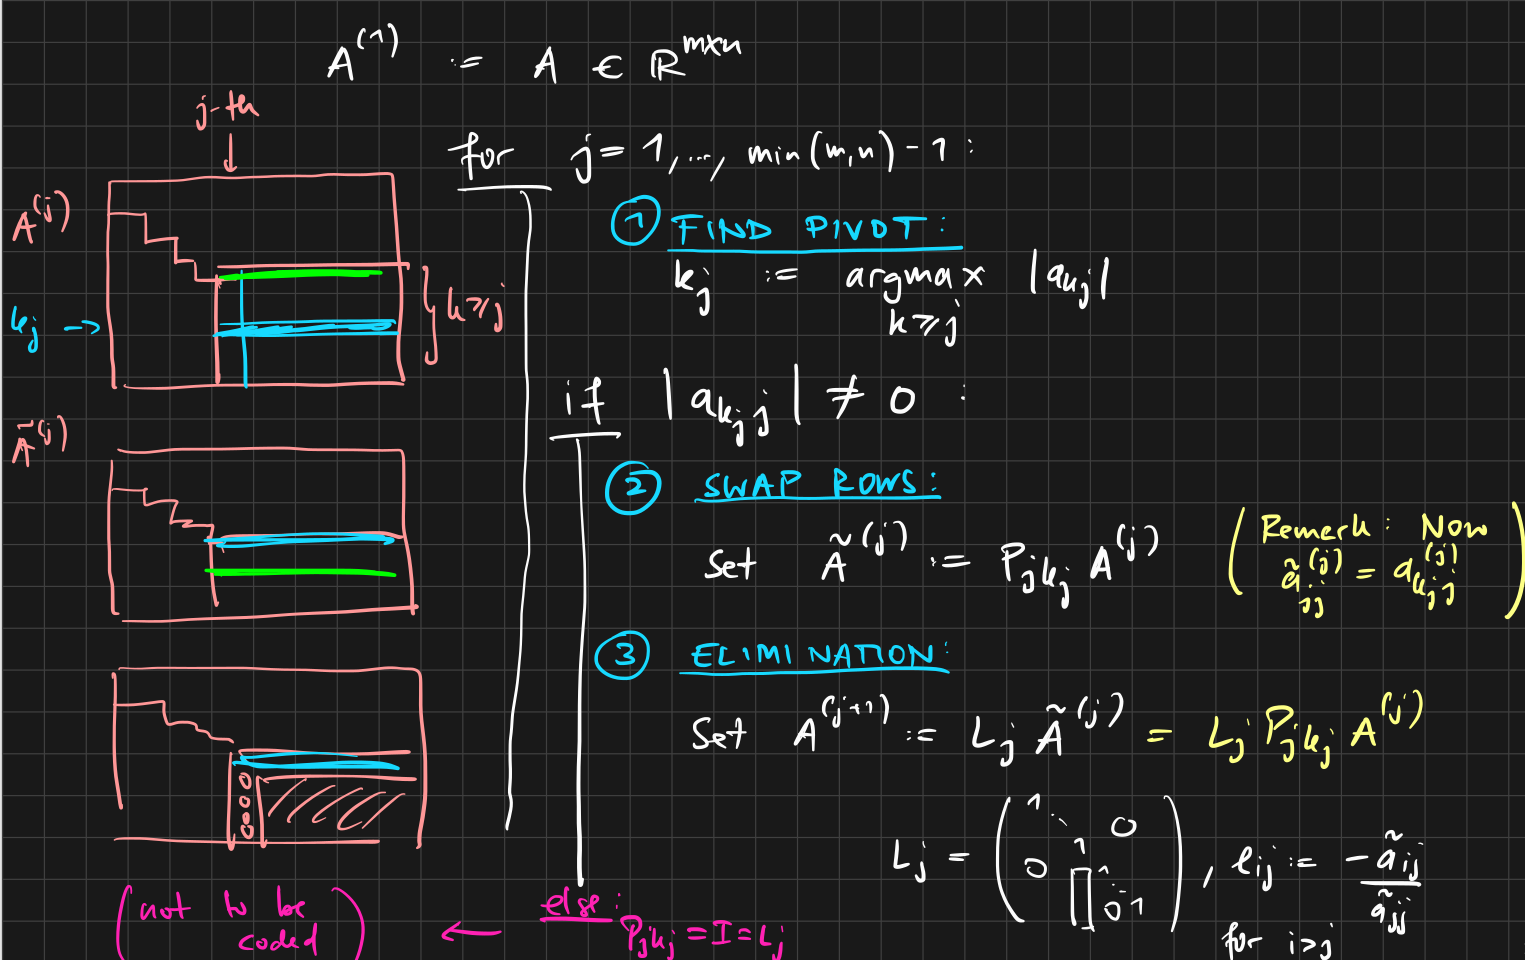
\includegraphics[width=0.9\textwidth]{gaussian-elimination.png}\\~\\~\\	
Remark: We can work \textit{in-place} and store numbers for $L$ and $U$ in the the same array.
		 }
	 
\end{frame}

\begin{frame}

	\textbf{\small In-place Gaussian Elimination with Row Pivoting} (for $m=n$)\\~\\
		\footnotesize
	\textbf{INPUT:} $A\in \mathbb{R}^{n \times n}$ (and $b \in \mathbb{R}^n$)\\
\textbf{OUTPUT:} LU decomposition $PA = LU$ (and if  $Ax = b$ is uniquely solvable the solution $x\in \mathbb{R}^n$)\\
\hspace*{1cm}\begin{algorithm}[H]
		{\color{gray}\texttt{\# \textbf{FACTORIZATION}}}\\
		initialize \texttt{piv = [1,2,...,n]}\\
		\For{$j = 1,...,n-1$}{
			{\color{gray}\texttt{\#  \textbf{Find the j-th pivot}}}\\
			$k_j := \arg \max_{k\geq j} |a_{kj}|$ \label{pivot}\\
			\If{$a_{k_jj}\neq 0$}{
				{\color{gray}\texttt{\# \textbf{Swap rows}}}\\
				A[$k_j$,:] $\leftrightarrow$ A[j,:]\\
				{\color{gray}\texttt{\#  by hand we also transform b on the fly}}\\
				b[$k_j$] $\leftrightarrow$ b[j]\\
				\texttt{piv}[$k_j$] $\leftrightarrow$ \texttt{piv}[j]\\
				{\color{gray}\texttt{\# \textbf{Elimination}}}\\
				\For{$k = j+1,\dots,n$}{
					$\ell_{kj} := a_{kj} / a_{jj}$\\
					$a_{kj} = \ell_{kj}$\\
					
					\For{$i = j+1,\ldots, n$}{
						$a_{ki} = a_{ki} - \ell_{kj} a_{ji}$\\
						
					}
					{\color{gray}\texttt{\#  by hand we also transform b on the fly}}\\
					($b_{k} = b_{k} - \ell_{kj} b_{j}$)
				}
			}
			
		}
		{\color{gray}\texttt{\# \textbf{SOLVE}}}\\
		$\ldots$
	\end{algorithm}
\end{frame}


\color{fontcolor}
\begin{frame}
	~\\
	As in the algorithm consider $A\in\mathbb{R}^{n \times n}$. Then the algorithm eventually leads to
	$$U:=A^{(n)}=L_{(n-1)}P_{(n-1)k_{(n-1)}}\dots L_3P_{3k_3}L_2P_{2k_2}L_1P_{1k_1}A.$$
	~\\
	By construction of the algorithm, $A^{(n)}=:U$ has row echelon form (no rigorous proof provided in this course).
	~\\
~\\
		\textbf{Question:}	Can we group all $L_i$ and $P_{ik_i}$ in such a way that $PA=LU$?\\
		\begin{lemma} \small
			Let $m\in\mathbb{N}$.  Let $P_{ik_i} \in \mathbb{R}^{m \times m}$ be the permutation matrix which results from interchanging the $i$-th and $k_i$-th column of the identity matrix in $\mathbb{R}^{m \times m}$, where $k_i \geq i$. Further for $\ell_j := (0,\ldots,0,\ell_{j+1,j},\ldots,\ell_{m,j})^\top\in\mathbb{R}^m$ and the $j$-th unit vector $e_j\in\mathbb{R}^m$, let $L_j := I + \ell_je_j^\top \in \mathbb{R}^{m\times m}$.
			Then show that for all $1 \leq j< i \leq k_i\leq m$ we have
			$$P_{ik_i} L_j = \widehat{L}_j P_{ik_i}$$
			where $\widehat{L}_j :=  I + (P_{ik_i}\ell_j)e_j^\top$.
		\end{lemma}
	\Hide{	\begin{proof}\small
		 We find
		 \begin{align*}
		 P_{ik_i} L_j
		 &=  P_{ik_i}\left(I + \ell_je_j^\top \right)\\
		 &=  P_{ik_i} +  P_{ik_i}\ell_je_j^\top \\
		 &=  P_{ik_i} +  P_{ik_i}\ell_je_j^\top {\color{cyan}P_{ik_i}^\top P_{ik_i} }\\
		 &= (I +  P_{ik_i}\ell_je_j^\top  P_{ik_i}^\top) P_{ik_i} \\
		 &= (I +  P_{ik_i}\ell_j{\color{cyan} (P_{ik_i}e_j)^\top}) P_{ik_i} .\\
		 &= (I +  P_{ik_i}\ell_j{\color{cyan}e_j^\top}) P_{ik_i} .
		 \end{align*}
		 Since $j~{\color{red}<} ~i \leq k_i$ we find that $P_{ik_i}e_j=e_j$, since only zeroes are swapped.
	\end{proof}
	}
\end{frame}

\begin{frame}
%				We show in the exercise:
%	$$P_{ik_i}L_j=\hat{L}_jP_{ik_i},~~~~1\leq j{\color{cyan}~ <~} i\leq k_i\leq m$$
%\Vspace{3cm}
	By applying this result multiple times, we obtain
\Hide{	\begin{align*}
	\underbrace{(\hat{L}_{n-1}\cdots \hat{L}_{2}\hat{L}_1)}_{=:\widehat{L}}&\underbrace{(P_{(n-1)k_{(n-1)}}\cdots P_{2k_2}P_{1k_1})}_{=:P}\cdot A=U\\
	&\stackrel{L:=\widehat{L}^{-1}}{\Leftrightarrow}~~\\
	&PA=LU.
	\end{align*}}
\end{frame}


\begin{frame}
	Summary: 
	{\bf \large Row echelon form and $LU$ decomposition} ~\\
	\begin{defi}[REF] 
		~\\
		\begin{itemize} 
		\item[a)] \textbf{Row elementary operations} are 
		\begin{itemize}
		\item[1)] add a nonzero multiple of one row to another
		\item[2)] swap two rows
		\end{itemize}
		\item[b)] A matrix is in \textbf{row echelon form (REF)} when it satisfies the following conditions:
		\begin{itemize}
		\item[1)] The first non-zero element in each row (called the leading entry) is in a column to the right of the leading entry in the previous row.
		\item[2)] Rows with all zero elements, if any, are below rows having a non-zero element.
		\end{itemize}
		\end{itemize}
	\end{defi}
	~\\
	By applying these types of operations we find: \vspace{-0.2cm}
	\begin{theo}[LU Decomposition]\label{REF}
		Every matrix $A\in\F^{m\times n}$ can be transformed to REF by row elementary operations. Thus there is a matrix $U\in\F^{m\times n}$ in REF, a lower triangular matrix $L\in GL(m,\F)$ with $\ell_{ij}=0,\forall j>i,$ and $\ell_{ii}=1,\forall i,$ and a permutation matrix $P\in GL(m,\F)$ with exactly one entry ``1'' in each row and column and zero otherwise, such that
		\[
		P\cdot A=L\cdot U.
		\]
	\end{theo}
	~\\
	Since triangular matrices are invertible if and only if the diagonal elements are nonzero, we find for the square case $m=n$, that:\vspace{-0.2cm}
	\begin{corollary}[Invertibility of $A$]\label{corREF}
	A matrix $A\in\F^{n\times n}$ is invertible, if and only if its REF $U\in\F^{n\times n}$ has a nonzero diagonal, i.e, $u_{ii}\neq 0, \forall i=1,\ldots ,n$.
	\end{corollary}
\end{frame}



%%%%%%%%%%%%%%%%%%%%%%%%%%%%%%%%%%%%%%%%%%
% RECAP ON EXAMPLE
%%%%%%%%%%%%%%%%%%%%%%%%%%%%%%%%%%%%%%%%%
%\elomath{
%\begin{frame}
%\textbf{Recap example from above}:\\
%	{\blank
%		 
%		$\textcolor{orange}{ L_2}\underbrace{\textcolor{cyan}{P_{23}}\textcolor{orange}{L_1}}_{=\hat{L}_1P_{23}} \textcolor{cyan}{P_{13}} A = U$\\
%		\underline{j=1:}
%		\begin{align*}
%		\left(
%		\begin{array}{ccc|c}
%		0&2&3&2\\
%		1&3&5&4\\
%		2&4&6&6
%		\end{array}
%		\right)
%		\textcolor{cyan}{
%			\begin{bmatrix}
%			1\\2\\3
%			\end{bmatrix}
%		}
%		\stackrel{\text{I}\leftrightarrow\text{III}}{\rightsquigarrow}
%		\left(
%		\begin{array}{ccc|c}
%		2&4&6&6\\
%		1&3&5&4\\
%		0&2&3&2
%		\end{array}
%		\right)
%		\textcolor{cyan}{
%			\begin{bmatrix}
%			3\\2\\1
%			\end{bmatrix}
%		}
%		&\stackrel{\text{II'=II}-\frac{1}{2}\text{I}}{\rightsquigarrow}
%		\left(
%		\begin{array}{ccc|c}
%		2&4&6&6\\
%		\textcolor{orange}{\frac{1}{2}}&1&2&1\\
%		\textcolor{orange}{0}&2&3&2
%		\end{array}
%		\right)
%		\textcolor{cyan}{
%			\begin{bmatrix}
%			3\\2\\1
%			\end{bmatrix}
%		}\\
%	{\cyan 
%	P_{13}=\begin{pmatrix}
%	0&0&1\\
%	0&1&0\\
%	1&0&0
%	\end{pmatrix}}\hspace{2.5cm}
%&{\red L_1=\begin{pmatrix}
%	1&0&0\\
%	-\frac{1}{2}&1&0\\
%	0&0&1
%	\end{pmatrix}}
%		\end{align*}
%		\underline{j=2:}
%\begin{align*}
%\stackrel{\text{II}\leftrightarrow\text{III}}{\rightsquigarrow}
%\left(
%\begin{array}{ccc|c}
%2&4&6&6\\
%\textcolor{orange}{0}&2&3&2\\
%\textcolor{orange}{\frac{1}{2}}&1&2&1
%\end{array}
%\right)
%\textcolor{cyan}{
%	\begin{bmatrix}
%	3\\1\\2
%	\end{bmatrix}
%}
%&\stackrel{\text{III'=III}-\frac{1}{2}\text{II}}{\rightsquigarrow}
%\left(
%\begin{array}{ccc|c}
%2&4&6&6\\
%\textcolor{orange}{0}&2&3&2\\
%\textcolor{orange}{\frac{1}{2}}&\textcolor{orange}{\frac{1}{2}}&\frac{1}{2}&0
%\end{array}
%\right)
%\textcolor{cyan}{
%	\begin{bmatrix}
%	3\\1\\2
%	\end{bmatrix}
%}
%\begin{matrix}
%\Rightarrow~x_1=1\\
%\Rightarrow~x_2=1\\
%\Rightarrow~x_3=0
%\end{matrix}\\
%{\cyan 
%	P_{23}=\begin{pmatrix}
%	1&0&0\\
%	0&0&1\\
%	0&1&0
%	\end{pmatrix}}\hspace{2.5cm}
%&{\red L_2=\begin{pmatrix}
%	1&0&0\\
%	0&1&0\\
%	0&-\frac{1}{2}&1
%	\end{pmatrix}}
%\end{align*}
%	}
%\end{frame}
%
%\begin{frame}
%	~\\
%	{\blank
%		We find:
%		\begin{align*}
%		&\textcolor{orange}{
%			L=\begin{pmatrix}
%			1&0&0\\
%			0&1&0\\
%			\frac{1}{2}&\frac{1}{2}&1
%			\end{pmatrix}},
%		%
%		U=\begin{pmatrix}
%		2&4&6\\
%		0&2&3\\
%		0&0&\frac{1}{2}
%		\end{pmatrix},
%		%
%		\textcolor{cyan}{
%			P=\begin{pmatrix}
%			0&0&1\\
%			1&0&0\\
%			0&1&0
%			\end{pmatrix}}\\
%		%
%		&\textcolor{orange}{L}U=\begin{pmatrix}
%		1&0&0\\
%		0&1&0\\
%		\frac{1}{2}&\frac{1}{2}&1
%		\end{pmatrix}
%		\begin{pmatrix}
%		2&4&6\\
%		0&2&3\\
%		0&0&\frac{1}{2}
%		\end{pmatrix}
%		=\begin{pmatrix}
%		2&4&6\\
%		0&2&3\\
%		1&3&5
%		\end{pmatrix}\\
%		%
%		&\textcolor{cyan}{P}A=\begin{pmatrix}
%		0&0&1\\
%		1&0&0\\
%		0&1&0
%		\end{pmatrix}
%		\begin{pmatrix}
%		0&2&3\\
%		1&3&5\\
%		2&4&6
%		\end{pmatrix}
%		=\begin{pmatrix}
%		2&4&6\\
%		0&2&3\\
%		1&3&5
%		\end{pmatrix}\\
%		&\Rightarrow~~PA=LU
%		\end{align*}
%	}
%\end{frame}
%%% END ELOMATH
%}



\begin{frame}
%	The so-called ``\textbf{direct}'' (= exact solution in finite steps) solution process for the system $Ax=b$ sketched above comprises two steps:~\\~\\
	\begin{itemize}
		\item[{\bf~(1)}] {\bf~Factorization:}~~~~{\tt Lu, Piv = scipy.linalg.lu\_factor(A)}~\\~\\
		\begin{itemize} \normalsize
			\item determine factors $L,U$ and permutation matrix $P$ such that $LU=PA$\\~\\
			\item the factors $L,U$ are compactly stored in one matrix {\tt Lu} $\in\R^{n\times n}$ of the same size as $A$ and the permutation matrix $P$ in CSR format as integer vector {\tt Piv} $\in\N^{n}$.
		\end{itemize} ~\\
		\vspace{0.8cm}
		\item[{\bf~(2)}] {\bf~Solution:}~~~~~~~~~~~{\tt x = scipy.linalg.lu\_solve((Lu, Piv), b)}~\\~\\
		\begin{itemize}
			\normalsize
			\item[\color{cyan}(2.1)] permute right-hand side $\bar{b}=Pb$~\\~\\
			\item[\color{cyan}(2.2)] solve lower triangular system $Lz=\bar{b}$ for $z$ (forward substitution)~\\~\\
			\item[\color{cyan}(2.3)] solve REF system $Ux=z$ for $x$  (backward substitution)
		\end{itemize}
	\end{itemize}
	~\\
	~\\
	Both, (1) and (2), are combined in the routine $${\tt x = scipy.linalg.solve(A,b)}.$$ 
	%
\end{frame}



 
\begin{frame}
\Subsubsection{Identify the number of solutions from the REF}~\\
%	\textbf{~Identify the number of solutions $|S|$ from the REF $U$}\\
% ~\\~\\
\Hide{ First, by inserting the $LU$ decomposition we obtain
	$$S:=\{x\in\mathbb{R}^n:~Ax=b\}\stackrel{A=P^TLU}{=}\{x\in\mathbb{R}^n:~P^TLUx=b\} = \{x\in\mathbb{R}^n:~Ux=\underbrace{L^{-1}Pb}_{=:z}\}.$$	
	~\\ \small
	Then we find for the three possible cases of the solution set (exercise):
	\begin{itemize}
		\item [1)] $U$ does not have a zero row (i.e., $m\leq n$)
			\begin{itemize}
				\item[1.1)] $m=n$: Then $U$ is invertible and $|S|=1$ with $x=U^{-1}L^{-1}Pb$
				\item[1.2)] $m<n$: Then has dependent columns but $\im(U)=\Rm$, so that $|S|=\infty$\\
				{\footnotesize\color{cyan}Note: The $m$ rows of $U$ are independent. Thus $m = \dim \im U^\top$. Also from dimension formula $ \dim \ker U^\top = m - \dim \im U^\top=0 $, so that $\ker U^\top = \{0\}$ and thus $\im(U) = (\ker U^\top)^\bot = \{0\}^\bot = \Rm$. }¸
			\end{itemize}
%		\item $U$ is invertible ($\Leftrightarrow m=n, ~u_{ii}\neq 0 \forall i$)\\
%		 $\Rightarrow~~|S|=1,~x=U^{-1}L^{-1}Pb$~\\~\\
		\item [2)] $U$ has at least one zero row
					\begin{itemize}
				\item [2.1)]
				For all zero rows in $U$, the transformed right-hand side $z$ is also zero there:\\
				$\Rightarrow~~Ux=z$ has infinitely many solutions, i.e., $|S|=\infty$\\
				~~~~~~(Note: $0x_1+\dots+0x_n=z_i=0$ is true for any $x$)~\\~\\
				\item [2.2)]
				else: $|S|=0$\\
				(Note: $0x_1+\dots+0x_n=z_i\neq0$ false for any $x$)~\\~\\
			\end{itemize}
%		\item $U$ is not invertible:
%		\begin{itemize}
%			\item [2.1)] $m\geq n$ and $U$ has at least one zero row:
%			\begin{itemize}
%				\item [2.1.1)]
%				For all zero rows in $U$, the transformed right-hand side $z$ is also zero there:\\
%				$\Rightarrow~~Ux=z$ has infinitely many solutions, i.e., $|S|=\infty$\\
%				~~~~~~(Note: $0x_1+\dots+0x_n=z_i=0$ is true for any $x$)~\\~\\
%				\item [2.2.2)]
%				else: $|S|=0$\\
%				(Note: $0x_1+\dots+0x_n=z_i\neq0$ true for no $x$)~\\~\\
%			\end{itemize}
%		  \item [2.2)] $m< n$: exercise?
%		\end{itemize}
	\end{itemize}
}
\end{frame}
 
 
%%%%%%%%%%%%%%%%%%%%%%%%%%%%%%%%%%%%%%%%%%
% ELOMATH: MORE ON LU
%%%%%%%%%%%%%%%%%%%%%%%%%%%%%%%%%%%%%%%%%
%\elomath{
%%%%%%%%%%%%%%%%%%%%%%%%%%%%%%%%%%%%%%%%%
% The Rank of $A$ from $U$
%%%%%%%%%%%%%%%%%%%%%%%%%%%%%%%%%%%%%%%%
%\begin{frame}
% \textbf{~The Rank of $A$ from $U$}\\
% 	\centering
% 	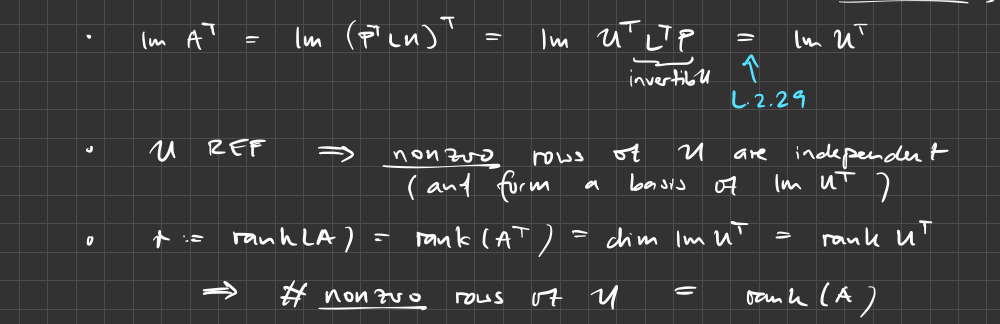
\includegraphics[width=0.9\linewidth]{lu-rank}
%\end{frame} 
% 


%%%%%%%%%%%%%%%%%%%%%%%%%%%%%%%%%%%%%%%%%
% Block Elimination and the Schur Complement
%%%%%%%%%%%%%%%%%%%%%%%%%%%%%%%%%%%%%%%%
%\begin{frame}
%	\Subsubsection{Block Elimination and the Schur Complement}
%		\centering
%		\Hide{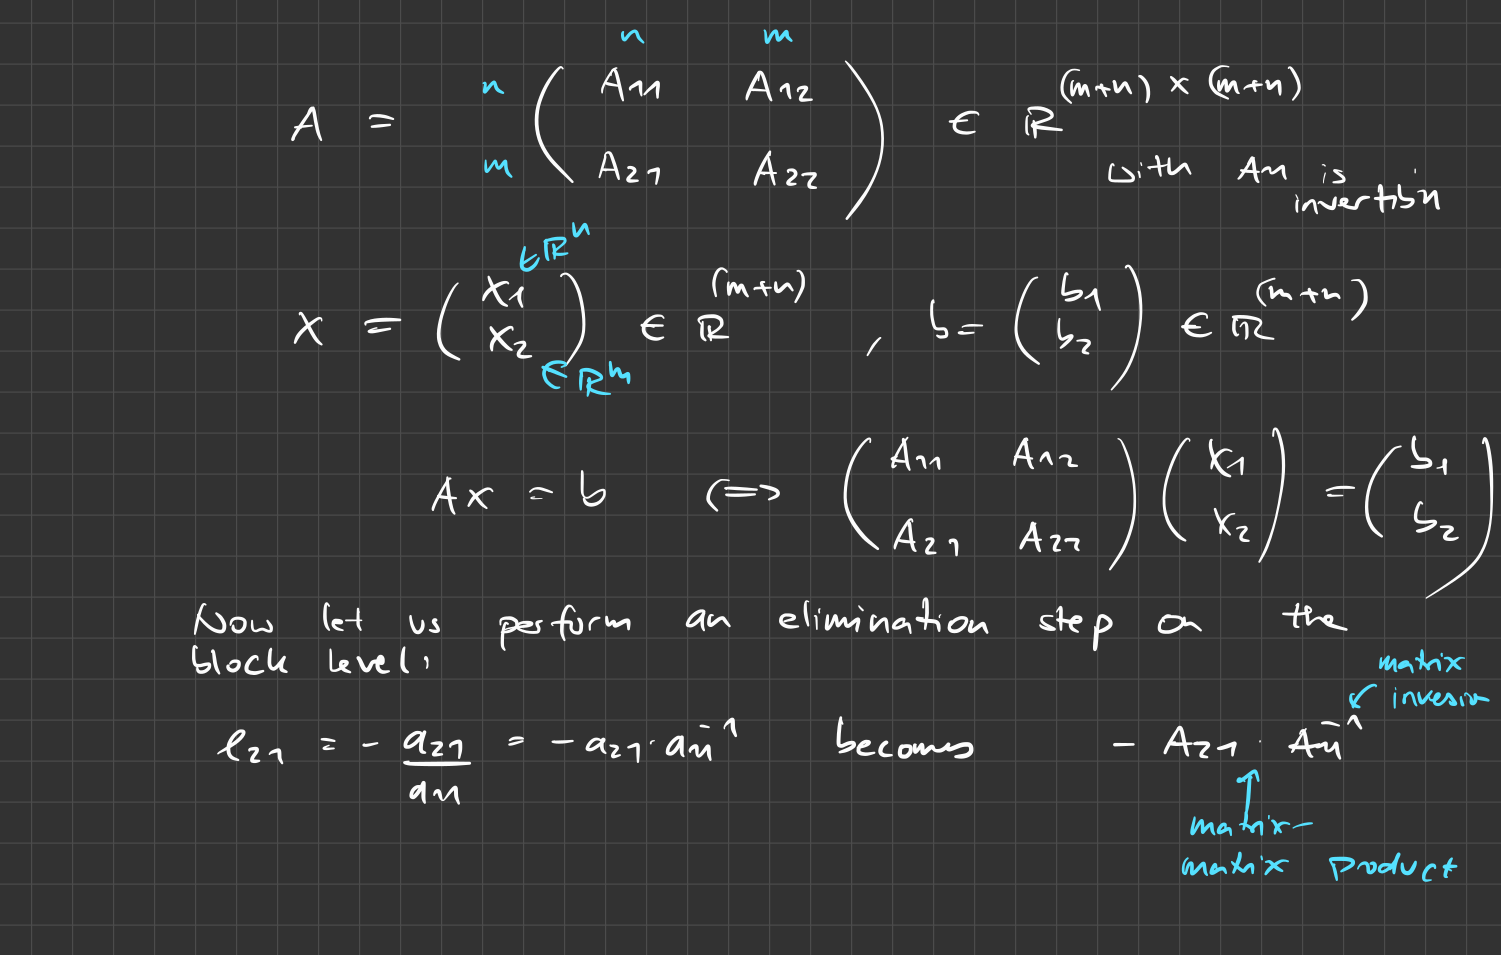
\includegraphics[width=0.9\linewidth]{lu-block1}}
%\end{frame}  
%\begin{frame}
%%	\textbf{~Block Elimination and the Schur Complement}\\
%		\centering
%		\Hide{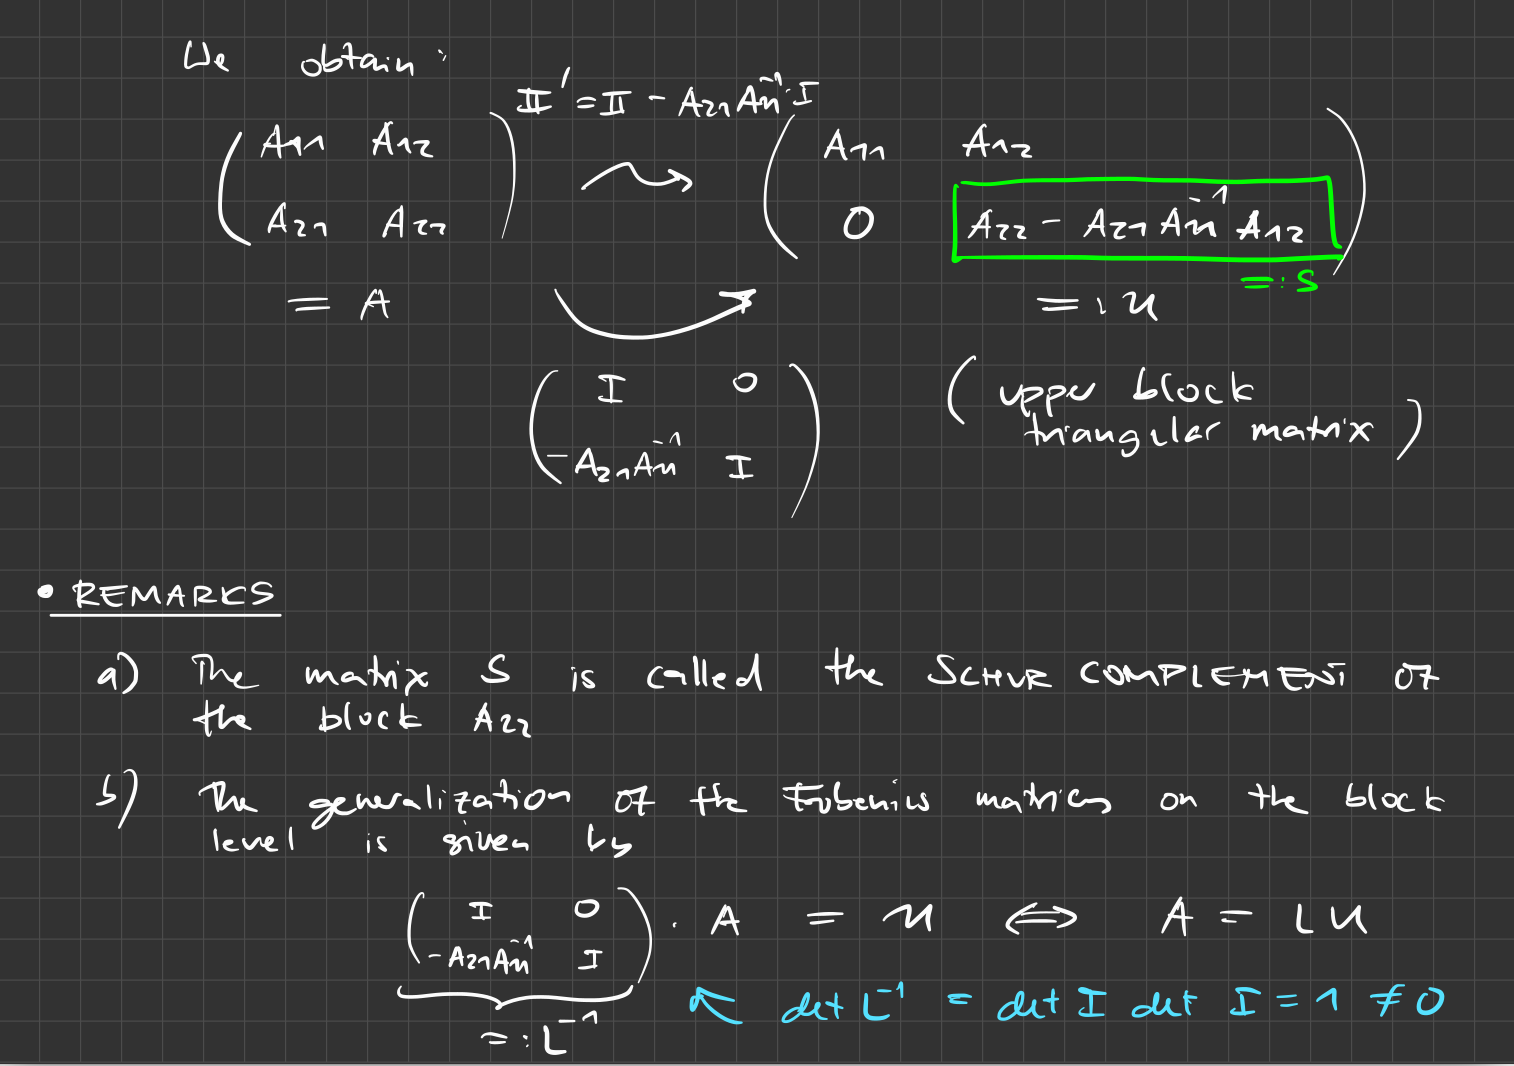
\includegraphics[width=0.9\linewidth]{lu-block2}}
%\end{frame}  
%\begin{frame}
%%	\textbf{~Block Elimination and the Schur Complement}\\
%	\centering
%		\Hide{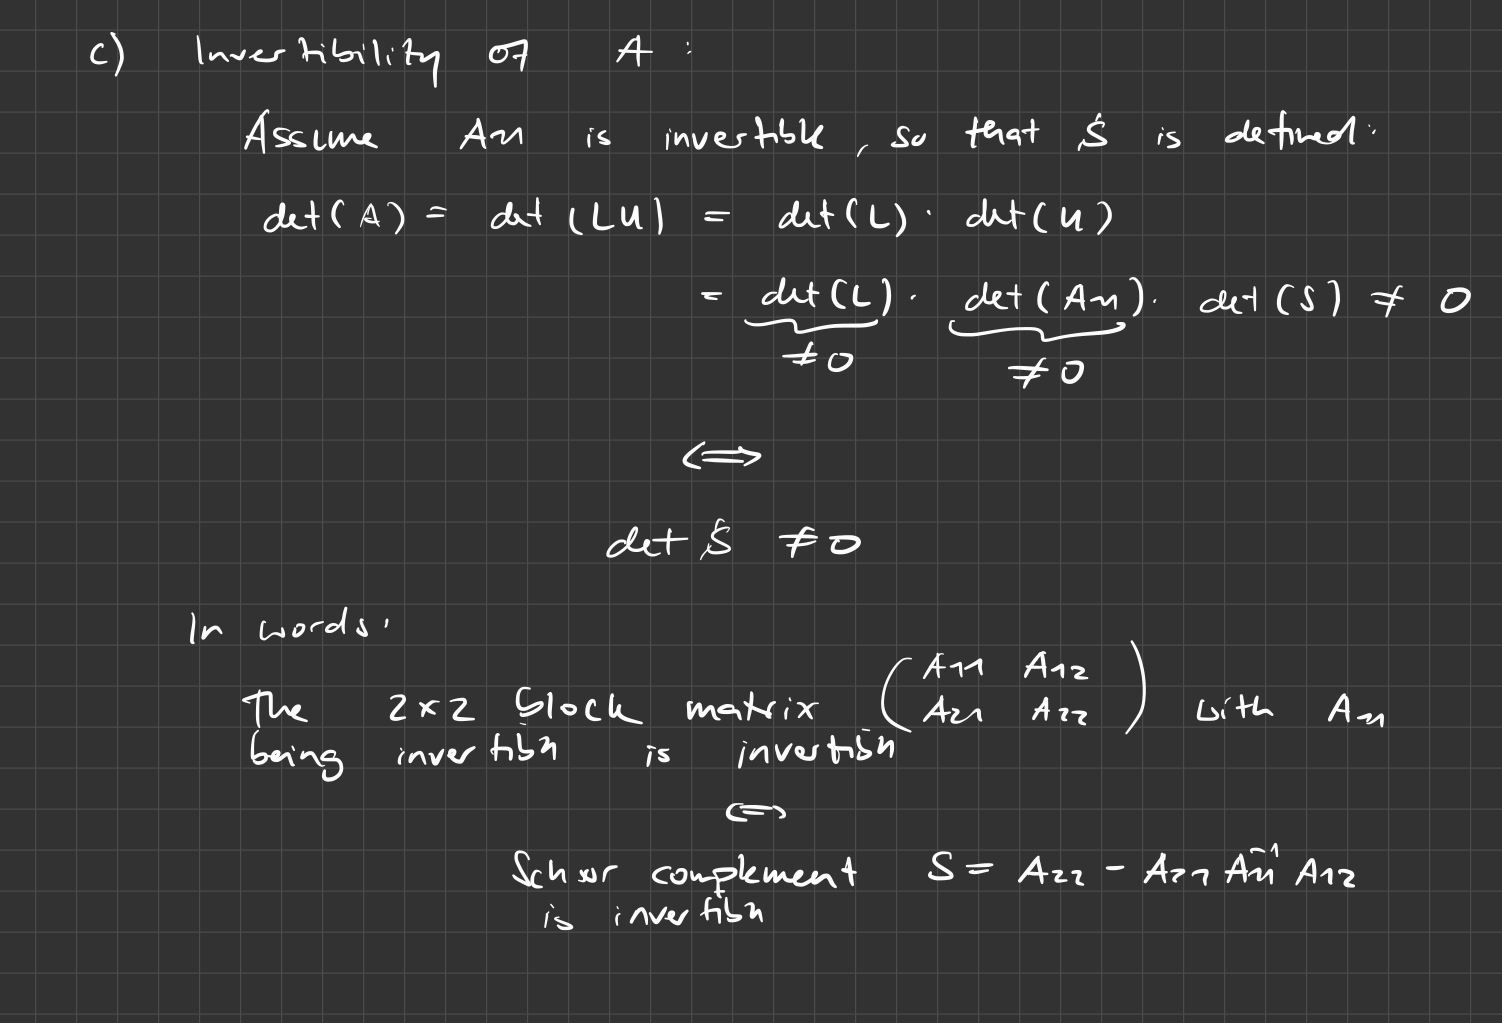
\includegraphics[width=0.9\linewidth]{lu-block3}}
%\end{frame}  
%\begin{frame}
%%	\textbf{~Block Elimination and the Schur Complement}\\
%		\centering
%		\Hide{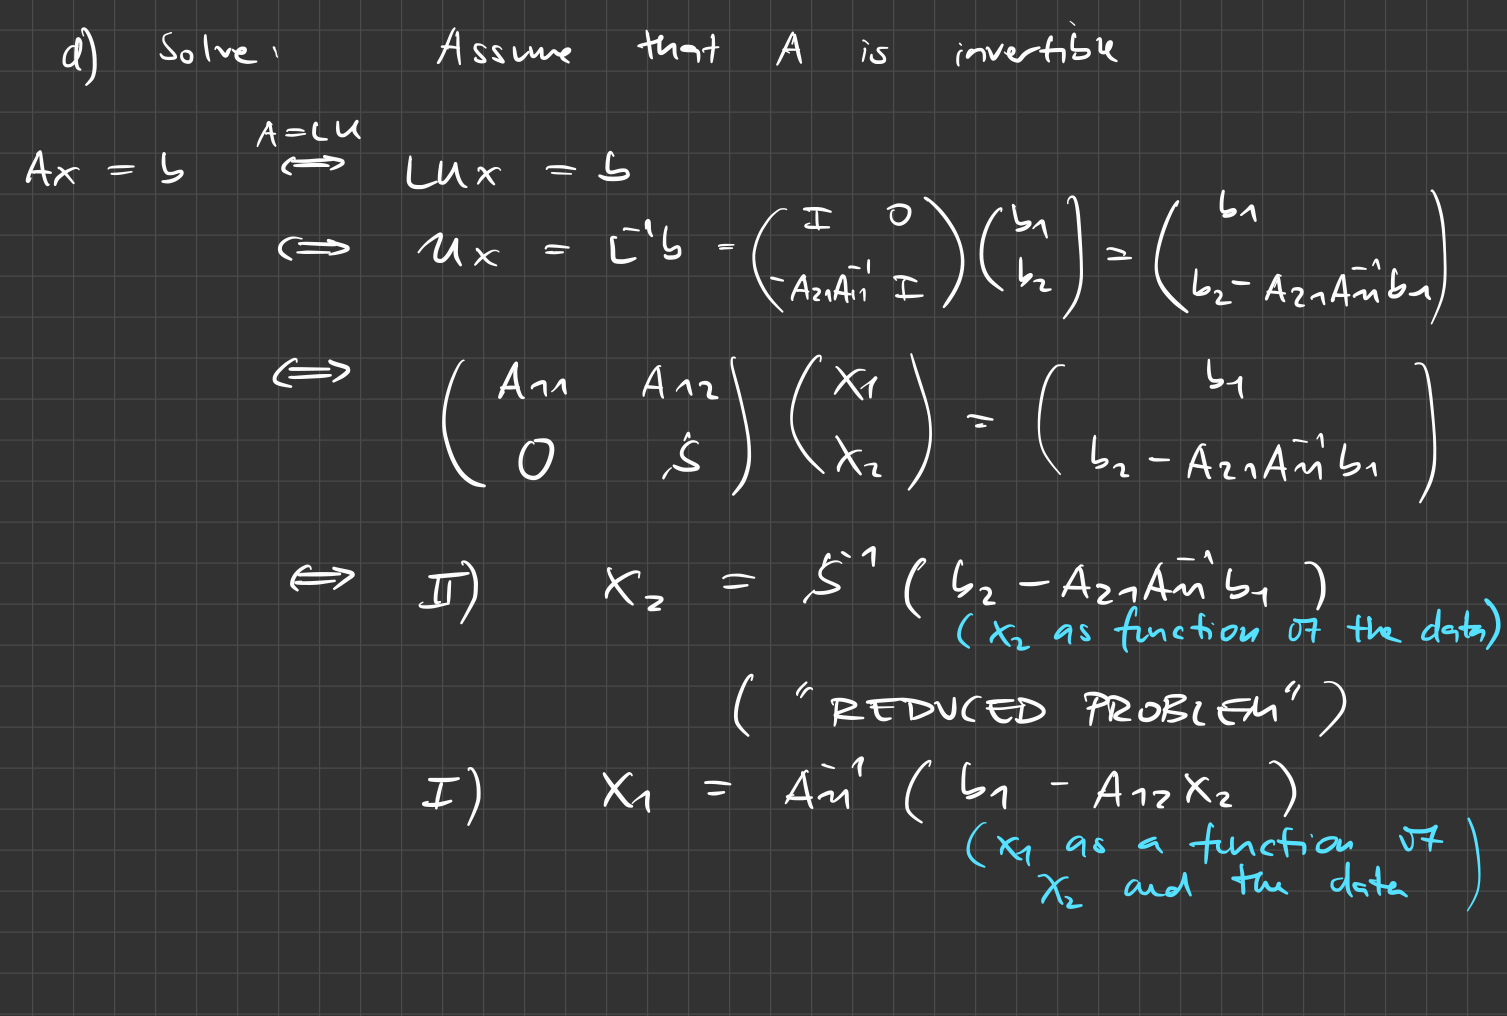
\includegraphics[width=0.9\linewidth]{lu-block4}}
%\end{frame}  


%%%%%%%%%%%%%%%%%%%%%%%%%%%%%%%%%%%%%%%%%
% Understanding Elimination as Substracting Rank-1 Pieces
%%%%%%%%%%%%%%%%%%%%%%%%%%%%%%%%%%%%%%%%
%\begin{frame}
%	\textbf{~Understanding Elimination as Substracting Rank-1 Pieces}\\
%		\centering
%	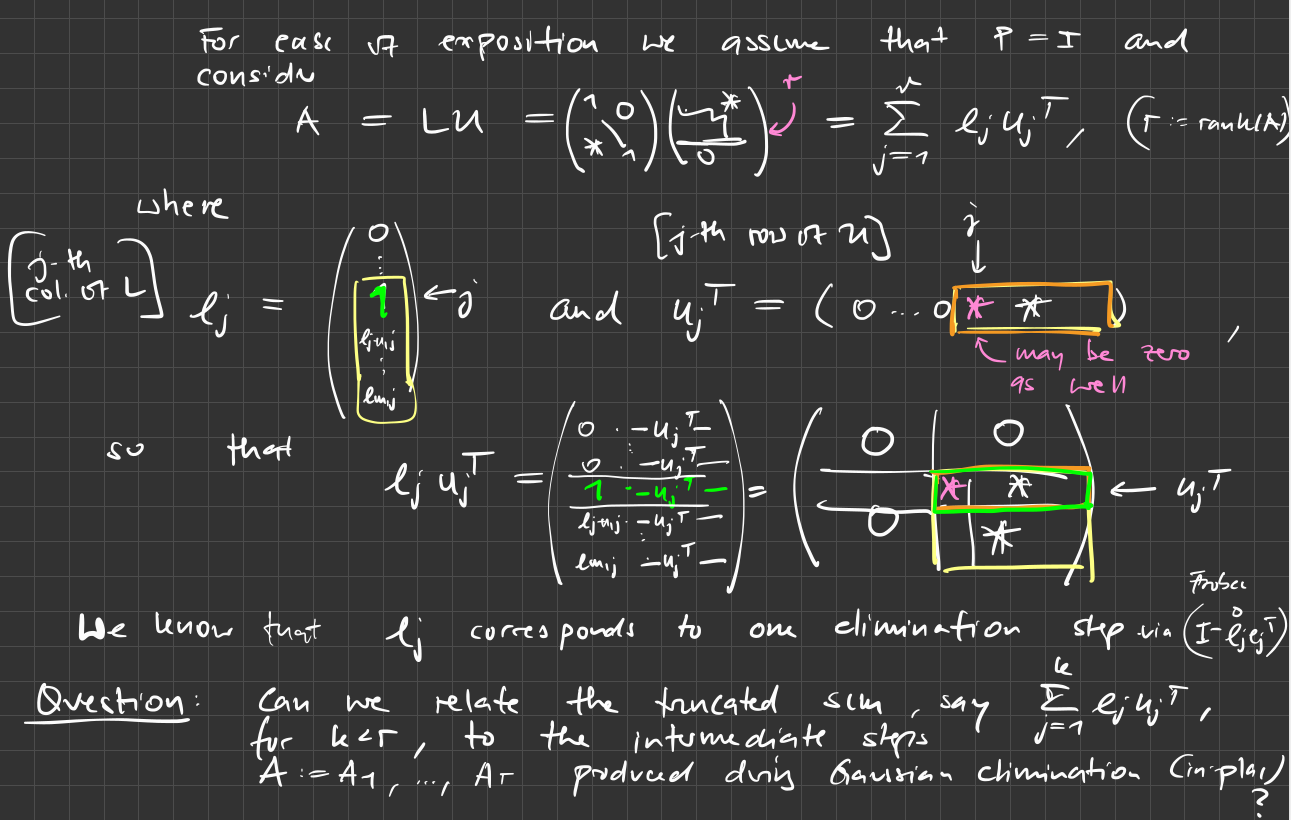
\includegraphics[width=0.95\linewidth]{lu-understanding-as-subs-rank1_1}
%\end{frame}  
%\begin{frame}
%	\centering
%	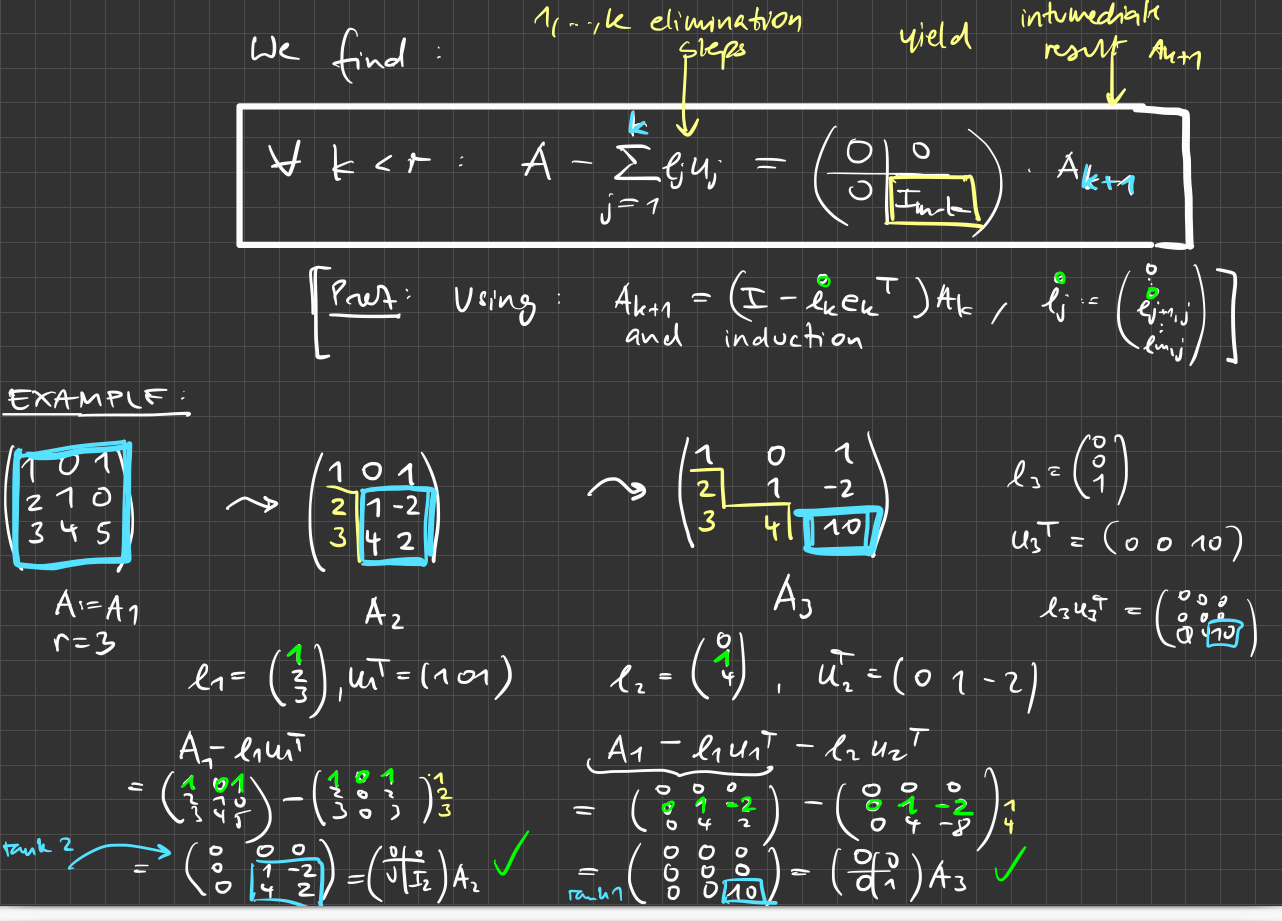
\includegraphics[width=0.95\linewidth]{lu-understanding-as-subs-rank1_2}
%\end{frame}  


%%%%%%%%%%%%%%%%%%%%%%%%%%%%%%%%%%%%%%%%%
% ROUNDING ERRORS
%%%%%%%%%%%%%%%%%%%%%%%%%%%%%%%%%%%%%%%%	
%\begin{frame}
%\Subsubsection{Pivoting to reduce rounding errors}	
%\Hide{
%	\begin{itemize}
%		\item In the above factorization procedure we went from column to column and eliminated the values under the diagonal element (the \textit{pivot element}). \vspace{0.2cm}
%		\item In order to reduce rounding errors one chooses the element in the current column which has largest absolute value as the pivot element (by permuting rows first).
%	\end{itemize}
%}
%\end{frame}
%\begin{frame}
%		~\\
%		\Hide{
%			\textbf{~Example} (rounding errors)\\
%			Let $\varepsilon\ll 1$ small enough, such that with machine precision
%			$$
%			{\yellow 1\pm \varepsilon =1}
%			$$
%			Consider
%			$$
%			A=\begin{pmatrix}
%			\varepsilon&2\\1&1
%			\end{pmatrix},
%			~b=\begin{pmatrix}
%			1\\1
%			\end{pmatrix}
%			~~\Rightarrow~~x_1=\frac{1}{2-\varepsilon}\approx\frac{1}{2},
%			~x_2=\frac{1-\varepsilon}{2-\varepsilon}\approx\frac{1}{2}
%			$$
%			Solve with elimination:\begin{itemize}
%				\item [1)]
%				\underline{No pivoting:}
%				\begin{align*}
%				&\left(
%				\begin{array}{cc|c}
%				\varepsilon&2&1\\
%				1&1&1
%				\end{array}
%				\right)
%				\stackrel{\text{II'=II}-\frac{1}{\varepsilon}\text{I}}{\rightsquigarrow}
%				\left(
%				\begin{array}{cc|c}
%				\varepsilon&2&1\\
%				0&1-\frac{2}{\varepsilon}&1-\frac{1}{\varepsilon}
%				\end{array}
%				\right)\\
%				\Rightarrow~~&x_2=\frac{1-\frac{1}{\varepsilon}}{1-\frac{2}{\varepsilon}}
%				=\frac{\varepsilon}{\varepsilon}\frac{1-\frac{1}{\varepsilon}}{1-\frac{2}{\varepsilon}}=\frac{\varepsilon-1}{\varepsilon-2}{\cyan\cong}\frac{1}{2}~~{\cyan(\text{machine precision})}\\
%				\Rightarrow~~&\varepsilon x_1+2\frac{1}{2}=1~~\Leftrightarrow~~x_1{\cyan\cong}0~~{\cyan(\text{machine precision})}
%				\end{align*}
%				\item [2)]
%				\underline{Pivoting:}
%				\begin{align*}
%				&\left(
%				\begin{array}{cc|c}
%				\varepsilon&2&1\\
%				1&1&1
%				\end{array}
%				\right)
%				\stackrel{\text{I}\leftrightarrow\text{III}}{\rightsquigarrow}
%				\left(
%				\begin{array}{cc|c}
%				1&1&1\\
%				\varepsilon&2&1
%				\end{array}
%				\right)
%				\stackrel{\text{II'=II}-\varepsilon\text{I}}{\rightsquigarrow}
%				\left(
%				\begin{array}{cc|c}
%				1&1&1\\
%				0&2-\varepsilon&1-\varepsilon
%				\end{array}
%				\right)\\
%				\Rightarrow~~&x_2=\frac{1-\varepsilon}{2-\varepsilon}{\cyan\cong}\frac{1}{2}~~{\cyan(\text{machine precision})}\\
%				\Rightarrow~~&x_1=1-x_2=\frac{1}{2}~~{\green\checkmark~\text{much better approximation}}
%				\end{align*}
%			\end{itemize}
%		}
%	\end{frame}	
%}




%%%%%%%%%%%%%%%%%%%%%%%%%%%%%%%%%%%%%%%%%
% CHOLESKY
%%%%%%%%%%%%%%%%%%%%%%%%%%%%%%%%%%%%%%%%
\begin{frame}[c]
	\hspace*{1.5cm}		\Subsection{The Cholesky Decomposition}
\end{frame}
	
\begin{frame}
	For symmetric and positive definite matrices $A\in \Rnn_{\text{spd}}\subset \text{GL}_n(\R)$ we obtain the following improvement:
	\begin{theorem}
		We have the equivalence
		$$A\in \Rnn_{\text{spd}} ~~\Leftrightarrow~~\exists_1~ L \in \Rnn \text{\emph{lower triangular}},~\ell_{ii}>0\colon~~ A = LL^\top.$$
	\end{theorem}
%	$$A=LL^T$$
%	for $L\in\Rnn$ being a lower triangular matrix (i.e., $U = L^\top$).
%	
~\\~\\
\begin{itemize}
	\item The Decomposition $A = LL^\top$ is called the \textbf{\color{defgruen} Cholesky decomposition of $A$}.
	\item Named after the french Mathematician André-Louis Cholesky (1875-1918) who developed this decomposition during his surveying work to solve the normal equation $A^\top A x = A^\top b$.
	\item We can derive an algorithm to compute the factor $L$.
	~\\~\\
	\item \textbf{Solving using $A=LL^\top$}\\
	$$Ax = b ~~\Leftrightarrow~~ LL^\top x = b ~~\Leftrightarrow~~ Lz = b,~~L^\top x = z~~~(\text{forward/backward Subst.})$$
\end{itemize}	
~\\~\\~\\
	\textit{In Python:}
	\begin{itemize}
		\item[{\bf~(1)}] {\bf~Factorization:}~~~~{\tt L, lower = scipy.linalg.cho\_factor(A)}~\\~\\
		\vspace{0.2cm}
		\item[{\bf~(2)}] {\bf~Solution:}~~~~~~~~~~~{\tt x = scipy.linalg.cho\_solve((L, lower), b)}
	\end{itemize}
\end{frame}
 
 
%%%%
% ELOMATH: More Remarks on Cholesky
%%%% 
%\elomath{
%\begin{frame}
%For the remainder, $A$ is assumed to be symmetric and positive definite.
%~\\~\\
%\textbf{~Remarks}
%\begin{itemize}
%	\item For $A \in \Rnn_{\text{spd}}$ we have $a_{ii} > 0$ (positive diagonal entries):\\
%	\Hide{~\\
%	For the unit vector $e_i$ we have $$a_{ii} = e_i^\top A e_i > 0. $$
%	~\\
%}
%\item \textbf{The $LDL$ Decomposition}\\~\\
%	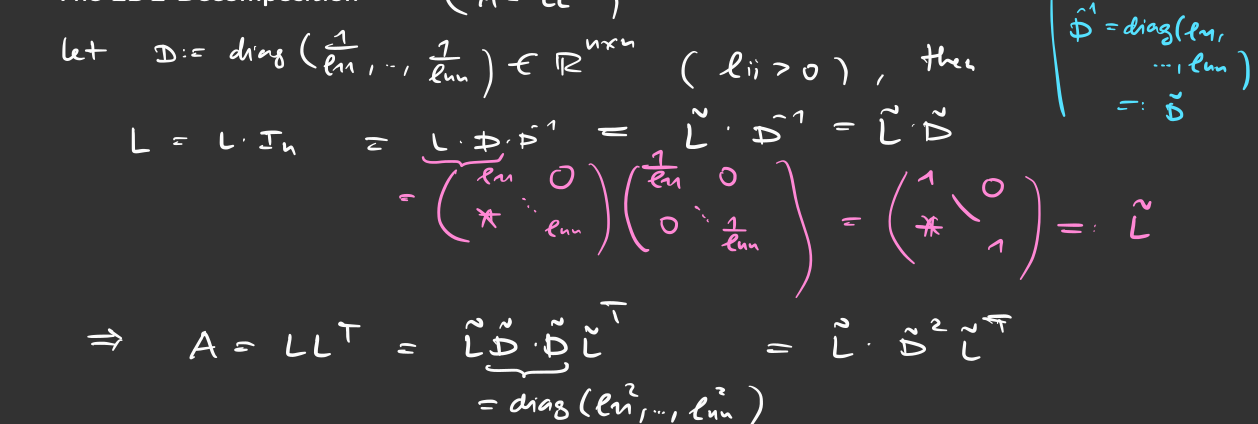
\includegraphics[width=0.9\linewidth]{cholesky-ldl}
%\end{itemize}
%\end{frame}
%\begin{frame}
%	\begin{itemize}
%		\item \textbf{The Determinant of $A$}\\~\\
%			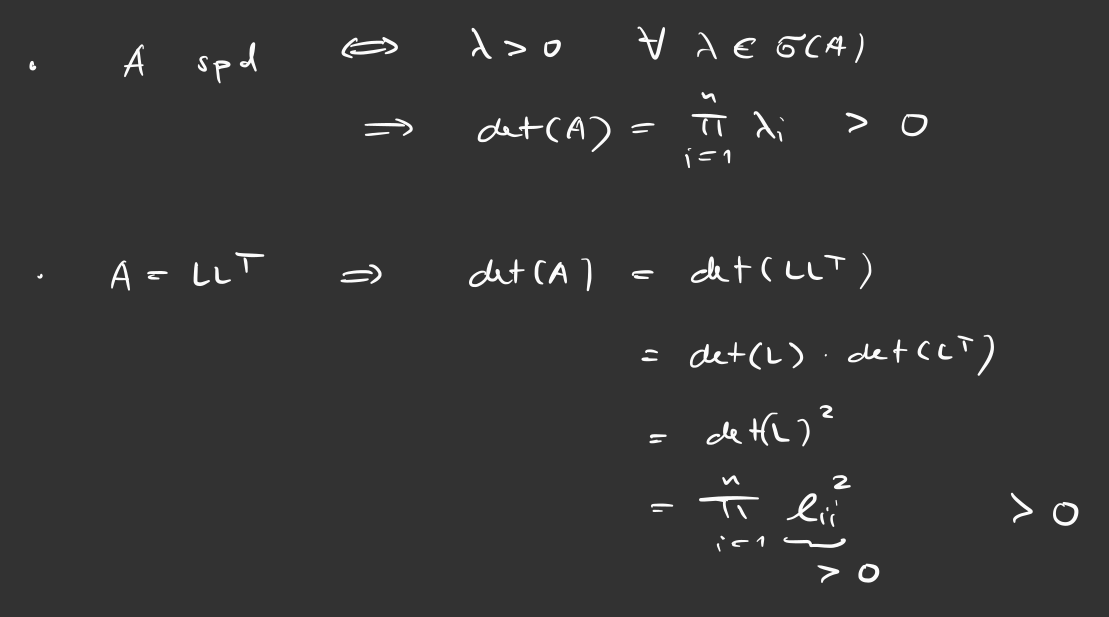
\includegraphics[width=0.99\linewidth]{cholesky-determinant}	
%	\end{itemize}
%\end{frame}
%\begin{frame}
%	\Subsubsection{Computation: ``Column by Column''}
%	By the theorem above we know that there exists an unique lower triangular matrix $L$ with positive diagonal entries $\ell_{ii} > 0$, so that
%	$$A= LL^\top.$$ 
%	By comparing each entry we obtain 
%	\Hide{~\\
%	\begin{align*}
%	a_{ik} = (LL^\top)_{ik} = \sum_{j=1}^n \ell_{ij}\underbrace{\widetilde{\ell}_{jk}}_{=\ell_{kj}} = \sum_{j=1}^n \ell_{ij}\underbrace{\ell_{kj}}_{=0,~k<j} = \sum_{j=1}^k\ell_{ij}\ell_{kj}
%	\end{align*}
%	~\\~\\~\\
%}	
%	From here we can now derive formulas for the entries $\ell_{ik}$ of $L$ which allow us to compute the matrix $L$ column by column.\\~\\ More precisely, for the $k$-th column of $L$ we obtain
%	\begin{itemize}
%		\item Above diagonal: $i<k$ ~\\
%		$$\ell_{ik} = 0 $$
%	\end{itemize}
%\end{frame}
%
%\begin{frame}
%	\Hide{~\\
%\begin{itemize}
%	\item Diagonal element: $i=k$
%    \item Below diagonal: $i>k$
%\end{itemize}
%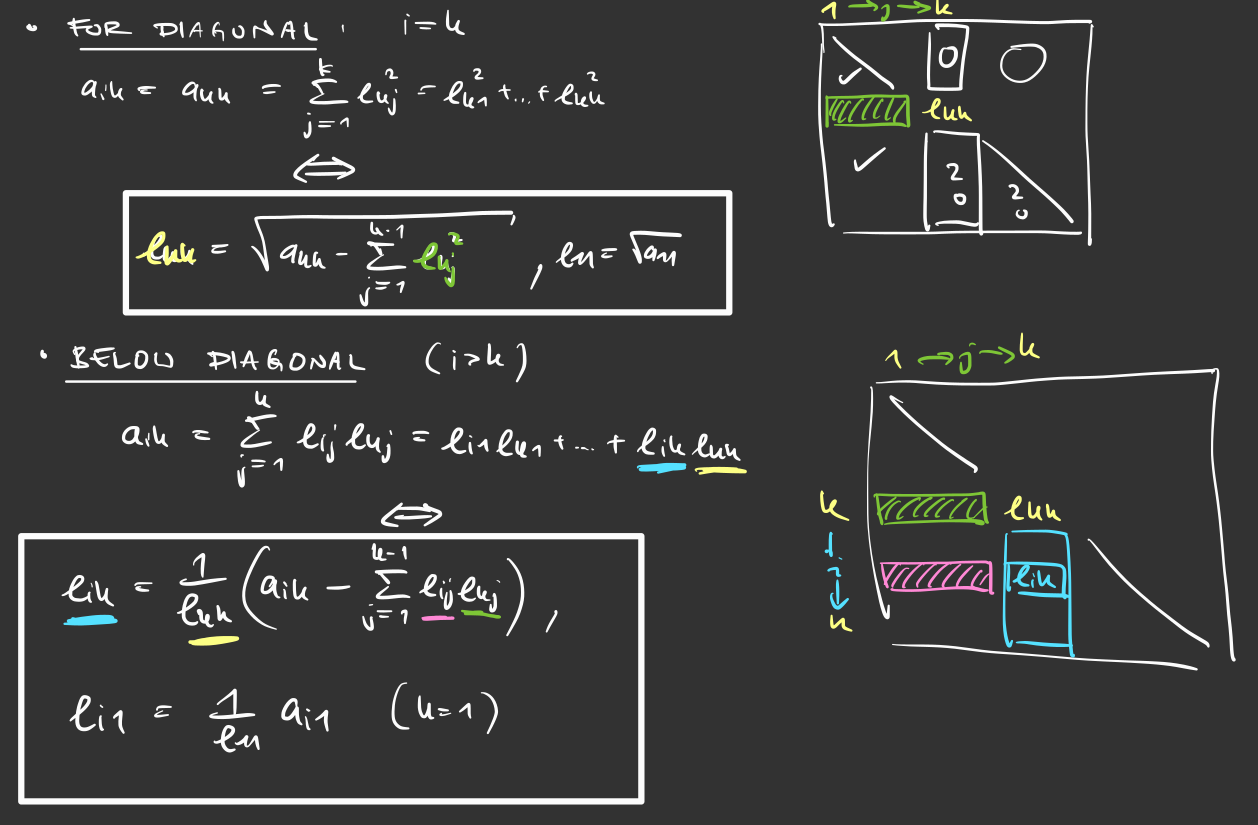
\includegraphics[width=0.99\linewidth]{cholesky-computation}
%~\\
%}
%\end{frame}
%
%\begin{frame}
%\textbf{~Remarks}\\~\\
%\begin{itemize}
%	\item The algorithm can work \textbf{in-place}: Once the data of a column of $A$ was accessed, it is no more needed in subsequent calculations.\\~\\
%	\item If, despite the symmetry of $A$, also the upper triangular part of $A$ was stored, then clearly this part needs to be zeroed at the end of the in-place algorithm.\\~\\
%	\item Using the algorithm as \textbf{test for the spd--property}:\\
%	The theorem tells us that $\ell_{ii}>0$; the algorithm computes $\ell_{ii}$. Thus, if we apply the algorithm to a matrix $A \in \Rnn$ and along the way we obtain $\ell_{ii} \leq 0$, then we know that the matrix is \textbf{not} positive definite.
%\end{itemize}	
%\end{frame}
%
%\begin{frame}
%	\Subsubsection{Comparison to Gaussian Elimination}
%	~\\
%	First note that 
%	$$A=LL^\top ~~\Leftrightarrow~~L^{-1} A = L^\top =~\text{upper triangular} $$
%	~\\
%	\begin{itemize}
%		\item $L^{-1}$ contains the ``elimination steps'' that transform $A$ into an upper triangular system.
%		\item However, here we can use a different approach to find the factors: Instead of applying row elementary operations we are able to derive closed formulas for $L$ directly from $A = LL^\top$ (since ``$U=L^\top$'').
%	\end{itemize}
%	~\\~\\
%	\textbf{Gaussian Elimination applied to a spd-Matrix}\\~\\
%	{\color{satzrot}\textbf{One can show:} For a symmetric and positive definite matrix $A$ there is no row pivoting needed (other than for stability reasons), i.e., there exist triangular matrices $L$ (lower) with 1's on the diagonal and $U$ (upper) so that $$A = LU.$$ }
%	\textbf{Question:} Is this the Cholesky decomposition? The answer is ``no'', which we will see in the example below.
%\end{frame}
% \begin{frame}
% 	\textbf{Example}\\~\\
% 	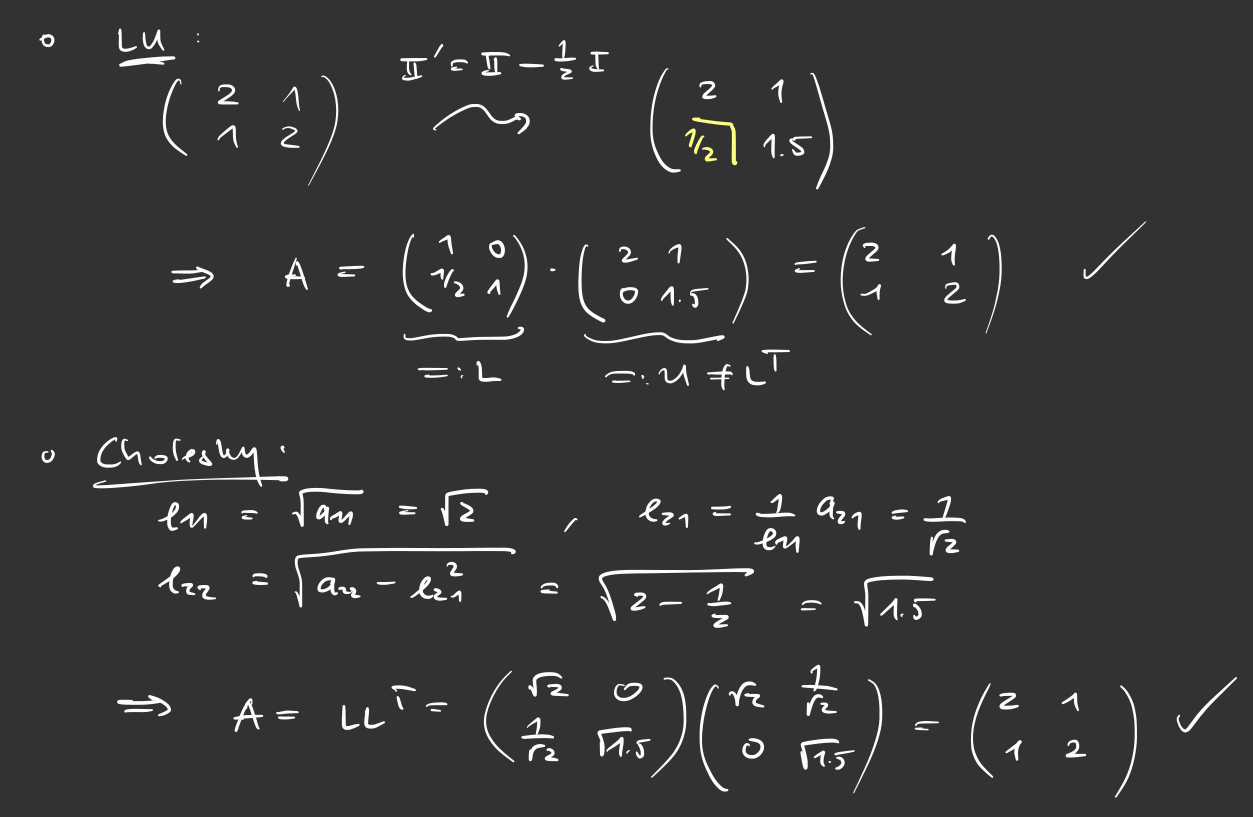
\includegraphics[width=0.99\linewidth]{cholesky-example}
% \end{frame}
%}

\begin{frame}
	\textbf{~Numerical Comparison: LU vs. Choleskly}\\~\\
	\begin{itemize}
		\item \textbf{Computational Costs:} ~\\The Cholesky decomposition is roughly twice as fast as Gaussian elimination (in terms of number of floating point operations). Clearly, we only need to compute one instead of two factors.\\~\\
		\item \textbf{Stability} (=``robustness against rounding errors'') :
		\begin{itemize}\normalsize
			\item Gaussian Elimination: Is only stable if a pivoting strategy is applied.
			\item Cholesky: Is stable even without pivoting.\\ (To avoid square roots, one can compute the LDL decomposition)
		\end{itemize}
	\end{itemize}
~\\~\\
\textbf{All in all:} \begin{center}
	\textit{For symmetric and positive definite matrices (of moderate size),\\ the Cholesky factorization is the preferred algorithm!}
\end{center}
\end{frame}


